% This example is meant to be compiled with lualatex or xelatex
% The theme itself also supports pdflatex
\PassOptionsToPackage{unicode}{hyperref}
\documentclass[aspectratio=1610, 12pt, xcolor=dvipsnames]{beamer}

% Warning, if another latex run is needed
% \usepackage[aux]{rerunfilecheck}

% just list chapters and sections in the toc, not subsections or smaller
\setcounter{tocdepth}{1}

%------------------------------------------------------------------------------
%------------------------------ Fonts, Unicode, Language ----------------------
%------------------------------------------------------------------------------
\usepackage{fontspec}
\defaultfontfeatures{Ligatures=TeX}  % -- becomes en-dash etc.

% german language
\usepackage{polyglossia}
\setdefaultlanguage{german}

% for english abstract and english titles in the toc
\setotherlanguages{english}

% intelligent quotation marks, language and nesting sensitive
\usepackage[autostyle]{csquotes}

% microtypographical features, makes the text look nicer on the small scale
\usepackage{microtype}

% colors and stuff
\usepackage{xcolor}
\usepackage[most]{tcolorbox}
% Here was colback=SpringGreen before but it is not finding the xcolor package
\tcbset{on line,
        boxsep=4pt, left=0pt,right=0pt,top=0pt,bottom=0pt,
        colframe=white,colback=green,
        highlight math style={enhanced}
        }
\newtcolorbox{mybox}[3][]
{
  colframe = #2!25,
  colback = #2!20,
  coltitle = #2!20!black,
  title = {#3},
  #1
}
%\colorlet{Green!40}
%------------------------------------------------------------------------------
%------------------------ Math Packages and settings --------------------------
%------------------------------------------------------------------------------

\usepackage{amsmath}
\usepackage{amssymb}
\usepackage{mathtools}
\usepackage{bbold}

% Enable Unicode-Math and follow the ISO-Standards for typesetting math
\usepackage[
  math-style=ISO,
  bold-style=ISO,
  sans-style=italic,
  nabla=upright,
  partial=upright,
]{unicode-math}
\setmathfont{Latin Modern Math}

% nice, small fracs for the text with \sfrac{}{}
\usepackage{xfrac}


%------------------------------------------------------------------------------
%---------------------------- Numbers and Units -------------------------------
%------------------------------------------------------------------------------

\usepackage[
  locale=DE,
  separate-uncertainty=true,
  per-mode=symbol-or-fraction,
]{siunitx}
\sisetup{math-micro=\text{µ},text-micro=µ}
% \sisetup{tophrase={{ to }}}
%------------------------------------------------------------------------------
%-------------------------------- tables  -------------------------------------
%------------------------------------------------------------------------------

\usepackage{booktabs}       % \toprule, \midrule, \bottomrule, etc

%------------------------------------------------------------------------------
%-------------------------------- graphics -------------------------------------
%------------------------------------------------------------------------------

\usepackage{graphicx}
%\usepackage{rotating}
\usepackage{grffile}
\usepackage{tikz}
\usepackage{circuitikz}
\usepackage{tikz-feynman}
\usepackage{subcaption}

% allow figures to be placed in the running text by default:
\usepackage{scrhack}
\usepackage{float}
\floatplacement{figure}{htbp}
\floatplacement{table}{htbp}

% keep figures and tables in the section
\usepackage[section, below]{placeins}

% smileys
\usepackage{MnSymbol,wasysym}

%------------------------------------------------------------------------------
%---------------------- customize list environments ---------------------------
%------------------------------------------------------------------------------

\usepackage{enumitem}
\usepackage{listings}
\usepackage{hepunits}

\usepackage{pdfpages}
%------------------------------------------------------------------------------
%------------------------------ Bibliographie ---------------------------------
%------------------------------------------------------------------------------

\setbeamertemplate{itemize/enumerate body begin}{\tiny}
\setbeamertemplate{itemize/enumerate subbody begin}{\tiny}
\setbeamertemplate{itemize/enumerate subsubbody begin}{\tiny}
\usepackage{moresize}

\usepackage[
  backend=biber,   % use modern biber backend
  autolang=hyphen, % load hyphenation rules for if language of bibentry is not
                   % german, has to be loaded with \setotherlanguages
                   % in the references.bib use langid={en} for english sources
]{biblatex}
\addbibresource{references.bib}  % the bib file to use
\DefineBibliographyStrings{german}{andothers = {{et\,al\adddot}}}  % replace u.a. with et al.


% Load packages you need here
% \usepackage{polyglossia}
% \setmainlanguage{german}

\usepackage{csquotes}


% \usepackage{amsmath}
% \usepackage{amssymb}
% \usepackage{mathtools}

\usepackage{hyperref}
\usepackage{bookmark}

% load the theme after all packages

\usetheme[
  showtotalframes, % show total number of frames in the footline
]{tudo}

% Put settings here, like
\unimathsetup{
  math-style=ISO,
  bold-style=ISO,
  nabla=upright,
  partial=upright,
  mathrm=sym,
}

% \setbeamertemplate{itemize item}{\scriptsize$\blacktriangleright$}
% \setbeamertemplate{itemize subitem}{\scriptsize$\blacktriangleright$}

%Titel:
\title{SciFi reconstruction and alignment}
%Autor
\author[N.Breer]{\textbf{Nils Breer} on behalf of the SciFi alignment and Reconstruction team}
%Lehrstuhl/Fakultät
\institute{SciFi general at 108th LHCb week - 5th june 2023}
%Titelgrafik muss ich einfueren!!!
%\titlegraphic{\includegraphics[width=0.3\textwidth]{content/Bilder/interferenz.jpg}}
\date{}

\begin{document}
\maketitle

\begin{frame}\frametitle{Reconstruction and alignment overview}
  \begin{columns}
    \begin{column}[c]{0.4\textwidth}
      \begin{itemize}
        \item \large $\bullet$\, Big SciFi alignment team this year
        \item $\bullet$\, Working in close contact with SciFi hit efficiency, timing, survey, data quality, sim+reco, RTA and early measurements
        \item \large Thanks everyone for your support and feedback!
      \end{itemize}
    \end{column}
    \begin{column}[c]{0.6\textwidth}
      \textbf{People working with SciFi}
      \textbf{align and calibration}
      \begin{columns}
          \begin{column}[c]{0.45\textwidth}
            \begin{itemize}
              \item $\bullet$\, Fred Blanc
              \item $\bullet$\, Jessy Daniel
              \item $\bullet$\, Zehua Xu
              \item $\bullet$\, Emmy Gabriel
              \item $\bullet$\, Louis Henry
              \item $\bullet$\, Nils Breer
              \item $\bullet$\, Giulia Tuci
              \item $\bullet$\, Laurent Dufour
            \end{itemize}
          \end{column}
          \begin{column}[c]{0.55\textwidth}
            \begin{itemize}
              \item $\bullet$\, Blake Leverington
              \item $\bullet$\, Wouter Hulsbergen
              \item $\bullet$\, Izaac Sanderswood
              \item $\bullet$\, Maria Vieites Diaz
              \item $\bullet$\, Mark Waterlaat
              \item $\bullet$\, Sophie Hollitt
              \item $\bullet$\, Miguel Ruiz Diaz
              \item $\bullet$\, Biljana Mitreska
            \end{itemize}  
          \end{column}
      \end{columns}      
    \end{column}
  \end{columns}
\end{frame}

\begin{frame}\frametitle{Overview of the topics}
  \begin{columns}
    \begin{column}[c]{0.33\textwidth}
      SciFi simulation and reconstruction
      \begin{itemize}
        \item $\bullet$\, Weekly group meeting: Monday, 13:15h
        \item $\bullet$\, Mailing list: lhcb-upgrade-ft-software
      \end{itemize}
      Alignment and Calibration
      \begin{itemize}
        \item $\bullet$\, Weekly group meeting: Tuesday, 11:00h
        \item $\bullet$\, Mailing list: lhcb-scifi-alignment-calib
      \end{itemize}
      \href{https://twiki.cern.ch/twiki/bin/view/LHCb/SciFiSimulation}{Twiki}
    \end{column}
    \begin{column}[c]{0.66\textwidth}
      \begin{itemize}
        \item \small $\bullet$\, Updates since \href{https://indico.cern.ch/event/1253790/}{last LHCb week}
        \begin{itemize}
          \item $\bullet$\, 2022 SciFi checks:
          \begin{itemize}
            \item - VELO drift studies
            \item - V3 SciFi alignment
            \item - $V^0$ studies of alignment versions
            \item - Stability measurements
          \end{itemize}
          \item $\bullet$\, Checks for 2023 alignments:
          \begin{itemize}
            \item - Survey and photogrammetry
      	    \item - Loose tracking and open VELO alignment
	          \item - New module constraint in progress 
          \end{itemize}
          Software and operations
          \begin{itemize}
            \item - Readout map development
            \item - Run control
          \end{itemize}
        \end{itemize}
        % \item $\bullet$\, gutes bild in lhcb week 106 von sophie
      \end{itemize}
    \end{column}
  \end{columns}
\end{frame}

\begin{frame}\frametitle{2022 VELO drift}
  \begin{columns}
    \begin{column}[c]{0.52\textwidth}
      \begin{figure}
        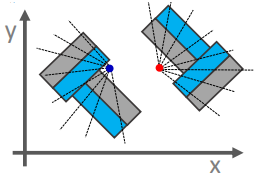
\includegraphics[width=0.6\textwidth]{plots/velo_axes.png}
        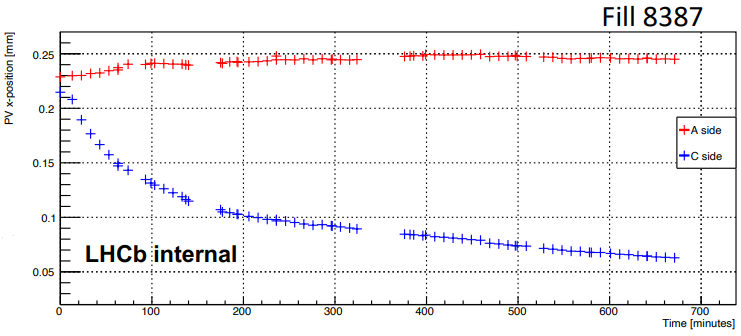
\includegraphics[width=0.9\textwidth]{plots/c_side_drift_freiss.png}
      \end{figure}
    \end{column}
    \begin{column}[c]{0.44\textwidth}
      \begin{itemize}
        \item $\bullet$\, The VELO drift has been confirmed with monitoring, alignment and material scan
        \item $\bullet$\, After the closing, C-side starts rotating around y with pivot point at around 850 mm
%        \item $\bullet$\, \to upstream region lacks behind
        \item $\bullet$\, Complications:
        \begin{itemize}
          \item $\bullet$\, Start of drift unpredictable
          \item $\bullet$\, Drift amount differs over time
        \end{itemize}
      \end{itemize}
      Also see \href{https://indico.cern.ch/event/1272210/contributions/5370939/attachments/2641017/4570404/2023_05_04_ASWeek_FReiss.pdf}{Florian's slides}
    \end{column}
  \end{columns}
\end{frame}

\begin{frame}\frametitle{VELO drift impact for SciFi alignment on 2022 data}
  \begin{columns}
    \begin{column}[c]{0.48\textwidth}
      \begin{itemize}
        \item $\bullet$\, Goal: estimate impact of VELO movement on reconstructed mass
        \item $\bullet$\, DoFs: Tx, Rz long modules aligned
        \item $\bullet$\, Data set: $\symup{B}^0 \to D^{*}\pi$ and $\symup{D}_0 \to \symup{K}\pi$
        \item $\bullet$\, Outcome: the mean value of the mass is consistent. 
        \item $\bullet$\, Resolution: got slightly worse but still within a standard deviation
      \end{itemize}
      

      Thanks to Miguel!
    \end{column}
    \begin{column}[c]{0.48\textwidth}
      \begin{figure}
        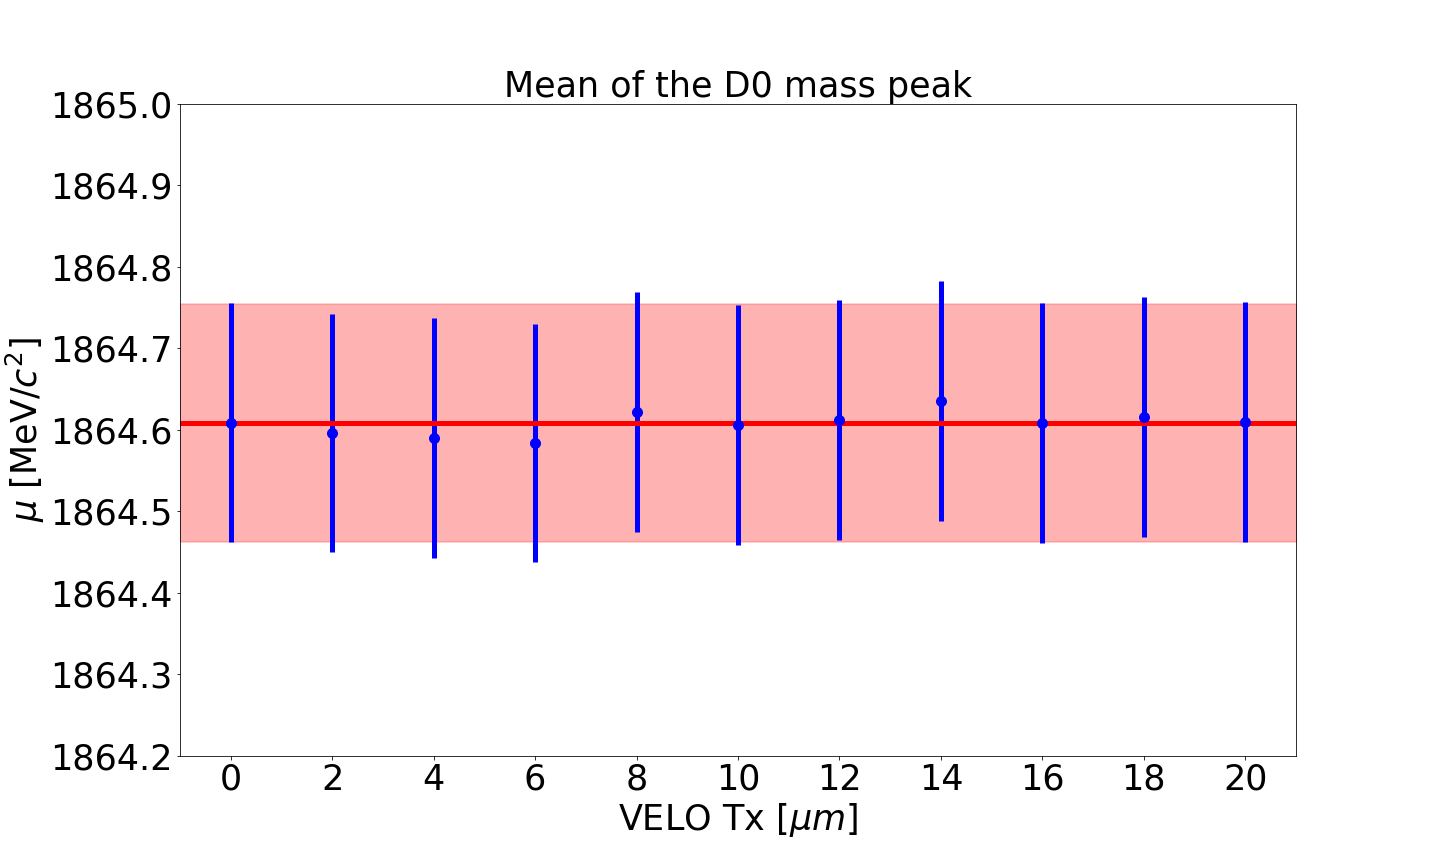
\includegraphics[width=0.5\textwidth]{reading_material/current_stuff/velo_drift_plots/plots/D0_massvalue_largeVPTx.png}
        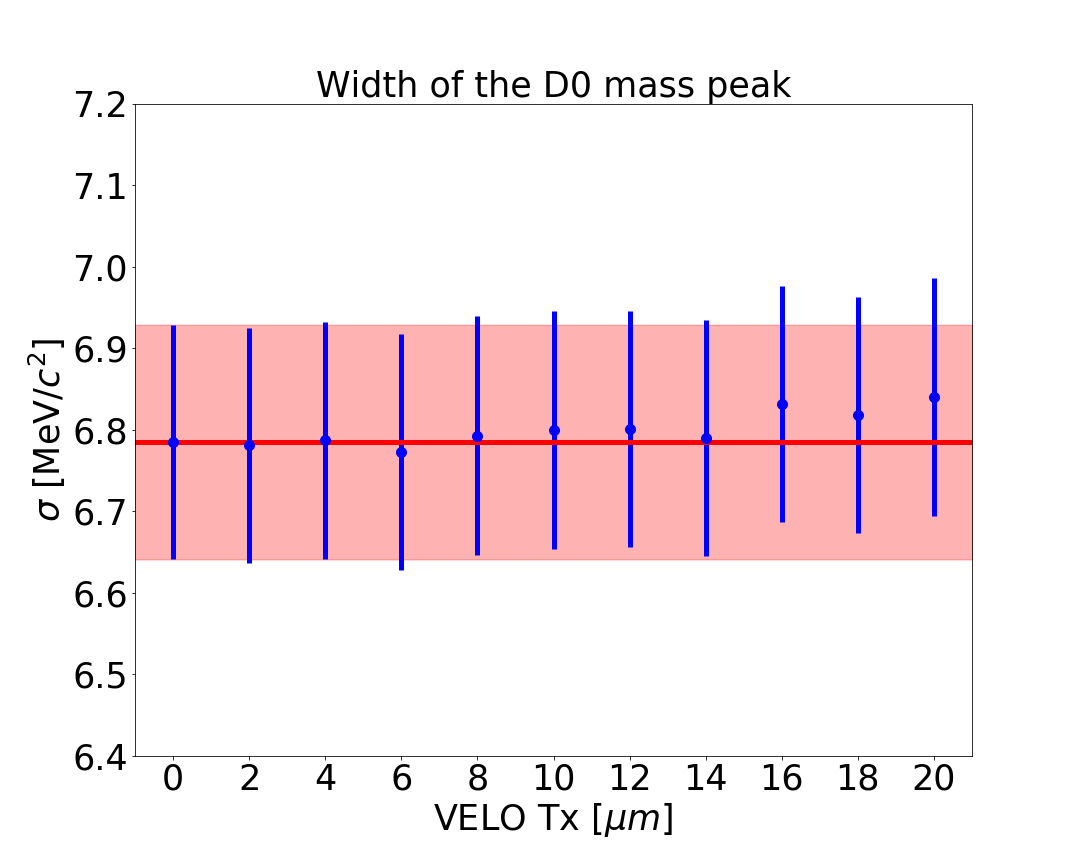
\includegraphics[width=0.5\textwidth]{reading_material/current_stuff/velo_drift_plots/plots/D0_resolution_smallVPTx.png}
        % 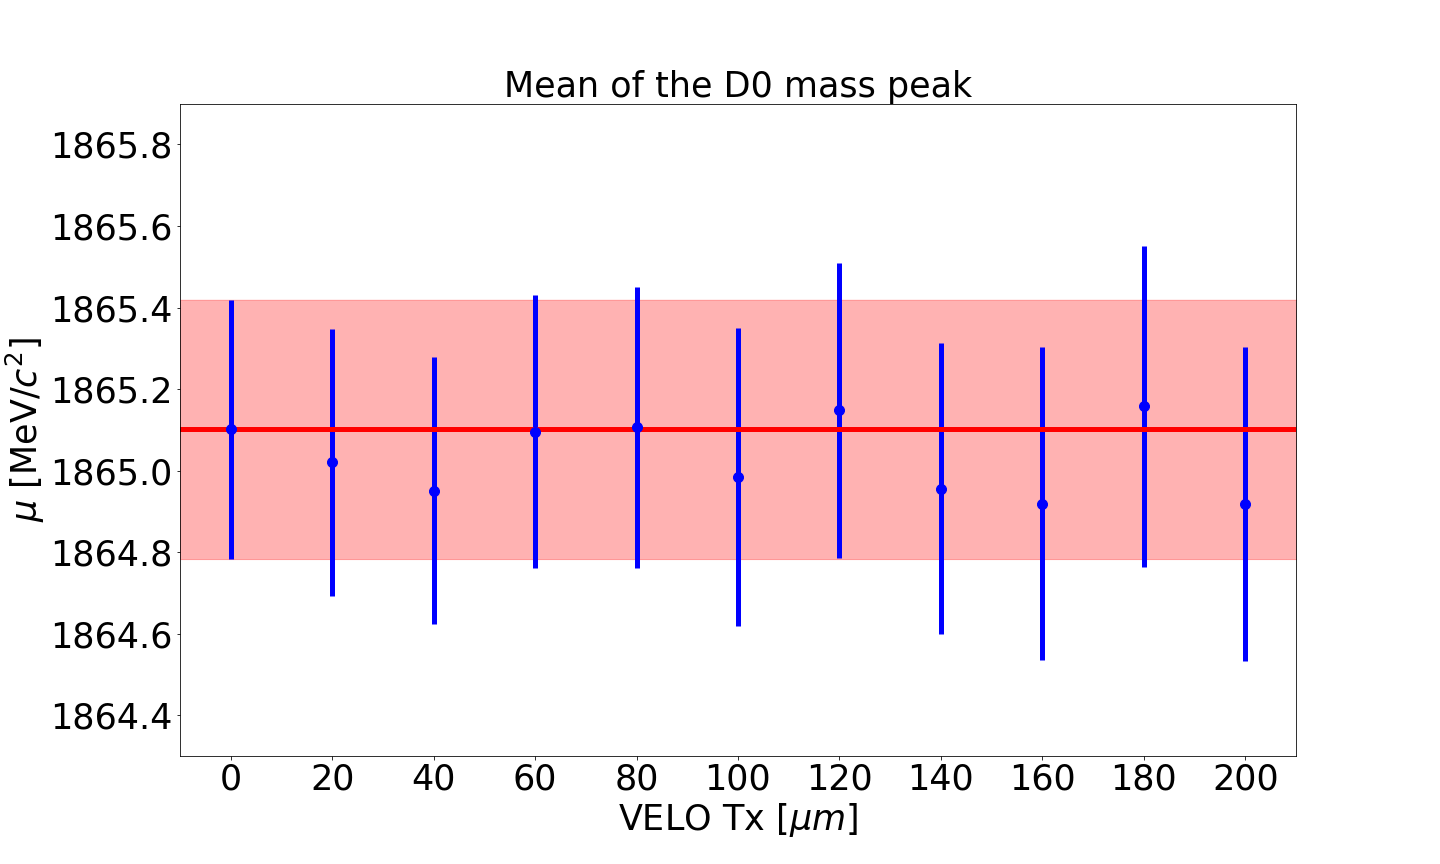
\includegraphics[width=0.5\textwidth]{reading_material/current_stuff/velo_drift_plots/plots/D0_massvalue_smallVPTx.png}
      \end{figure}
    \end{column}
  \end{columns}
\end{frame}

\begin{frame}\frametitle{SciFi alignment with 2022 data}
  \begin{columns}
    \begin{column}[c]{0.48\textwidth}
      \begin{figure}
        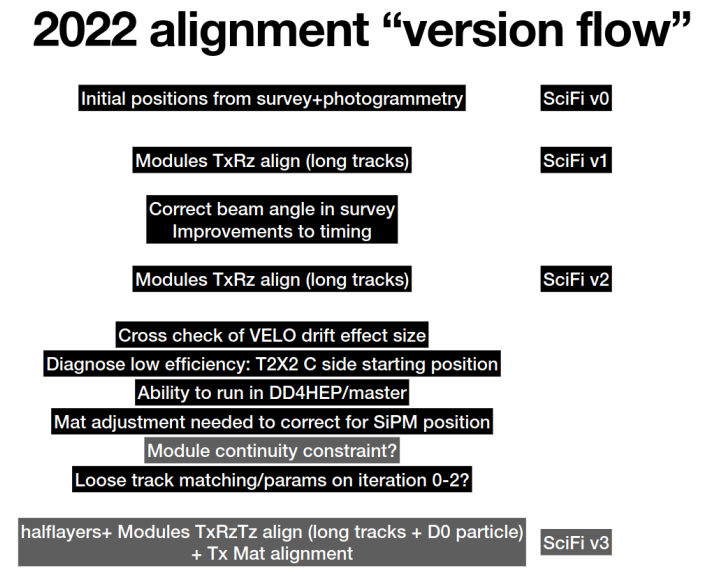
\includegraphics[width=0.9\textwidth]{plots/alignment_version_flow.png}
      \end{figure}
      from \href{https://indico.cern.ch/event/1275405/contributions/5372370/attachments/2636783/4562038/SciFiAlignUpdate_20230427.pdf}{Sophie's slides}
    \end{column}
    \begin{column}[c]{0.48\textwidth}
      \begin{itemize}
        \item $\bullet$\, Half modules to better correct for suboptimal starting conditions
        \item $\bullet$\, Beam angle fix + better fine timing
        \item $\bullet$\, Low efficiency C-side \to\, improved starting conditions
        \item $\bullet$\, Mats need to correct for SiPM positions
        \item $\bullet$\, Loose track matching/params in first iterations yield performance boost
        \item $\bullet$\, Final v3: TxTzRz, halflayers + modules, long tracks to D0 particles + Tx mat alignment
      \end{itemize}
    \end{column}
  \end{columns}
\end{frame}

\begin{frame}\frametitle{Overview of alignment v3 module}
 \begin{itemize}
	  \item $\bullet$\, Starts from 2022 SciFi survey positions unless otherwise marked
	  \item $\bullet$\, DD4Hep + PrKalman tracking
	  \item $\bullet$\, Run on 600k events (increased from 200k)
    \begin{itemize}
      \item $\bullet$\, All modules have sufficient statistics to align
    \end{itemize}
    \item $\bullet$\, Aligns in Tz degree of freedom (new since v2)
    \item $\bullet$\, Uses loose tracking mode (see \href{https://gitlab.cern.ch/lhcb/Moore/-/blob/master/Hlt/RecoConf/options/hlt2_loose_tracking_config.py}{setup}) and PatPV3D
    \item $\bullet$\, Uses D0 particle information (see \href{https://gitlab.cern.ch/lhcb/Alignment/-/blob/master/Alignment/Humboldt/python/Humboldt/ParticleSelections.py}{Selections})
    \item $\bullet$\, Constrained average Tx, Tz in SciFi backlayer
    \begin{itemize}
      \item $\bullet$\, Ideally allows us to compare alignments with shared momentum scale reference, prevent changes from curvature bias
      \item $\bullet$\, But this scale is not necessarily correct
    \end{itemize}
    \item $\bullet$\, These alignments shown consider modules only: mat alignment performed as a seperate step
  \end{itemize}
\end{frame}

\begin{frame}
  \begin{figure}
    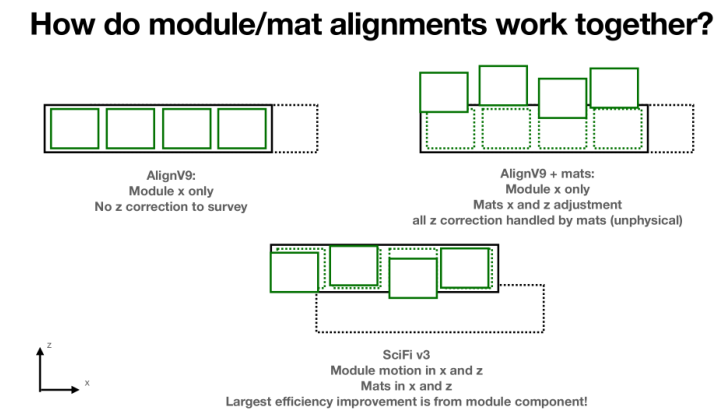
\includegraphics[width=0.9\textwidth]{plots/modules_and_mats.png}
    from \href{https://indico.cern.ch/event/1275394/contributions/5359493/attachments/2628409/4549668/SciFi_mat_alignment.pdf}{Zehua's slides}
  \end{figure}
\end{frame}

% \begin{frame}\frametitle{SciFi Mats: from v9 to v10}
%   \begin{columns}
%     \begin{column}[c]{0.48\textwidth}
%       \begin{figure}
%         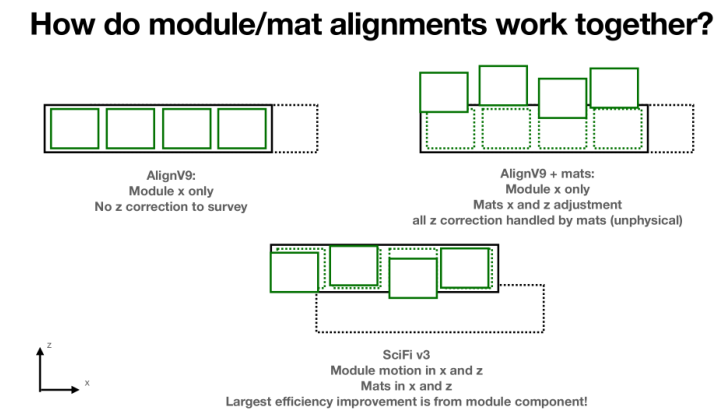
\includegraphics[width=\textwidth]{plots/modules_and_mats.png}
%       \end{figure}
%     \end{column}
%     \begin{column}[c]{0.48\textwidth}
%       \begin{itemize}
%         \item $\bullet$\, v9 featured no z correction in survey \to\, shifting of whole module in x
%         \item $\bullet$\, v9 + mats: SiPMs being aligned and not glued mats!
%         \item $\bullet$\, \to\, allowed unphysical movement out of the module
%         \item $\bullet$\, v10: modules movement in $x$ and $z$ allows for physical movement within module bounds
%         \item $\bullet$\, Yield: largest efficiency improvement from module alignment but mats needed
%       \end{itemize}
%     \end{column}
%   \end{columns}
% \end{frame}

\begin{frame}\frametitle{Mat alignment and the real SciFi}
  \begin{itemize}
    \item $\bullet$\, Real mats are glued together wth very fine tolerance/quality control (\approx \SI{50}{\micro\m}), but prelim mat alignment sees movement up to $\SI{1.5}{\milli\m}$
    \begin{itemize}
      \item $\bullet$\, "mat alignment" moves the mats in software to match the best hit position in tracking
      \begin{itemize}
        \item $\bullet$\, Depends on module alignment quality
        \item $\bullet$\, Depends on relative position of glued SiPM readouts relative to mats
      \end{itemize}
      \item $\bullet$\, Long term goal SciFi team: correct for hit positions in readout without moving mat material in simulation
      \begin{itemize}
        \item $\bullet$\, Understand rotations in survey positions that may produce z movement in reconstruction
        \item $\bullet$\, Understand true variations in SiPM positions
      \end{itemize}
      $\bullet$\, In the short term: offline mat alignment to improve reconstruction
    \end{itemize}
  \end{itemize}
\end{frame}

\begin{frame}\frametitle{Performance of v3 alignment on 2022 data}
  \begin{columns}
    \begin{column}[c]{0.49\textwidth}
      \begin{figure}
        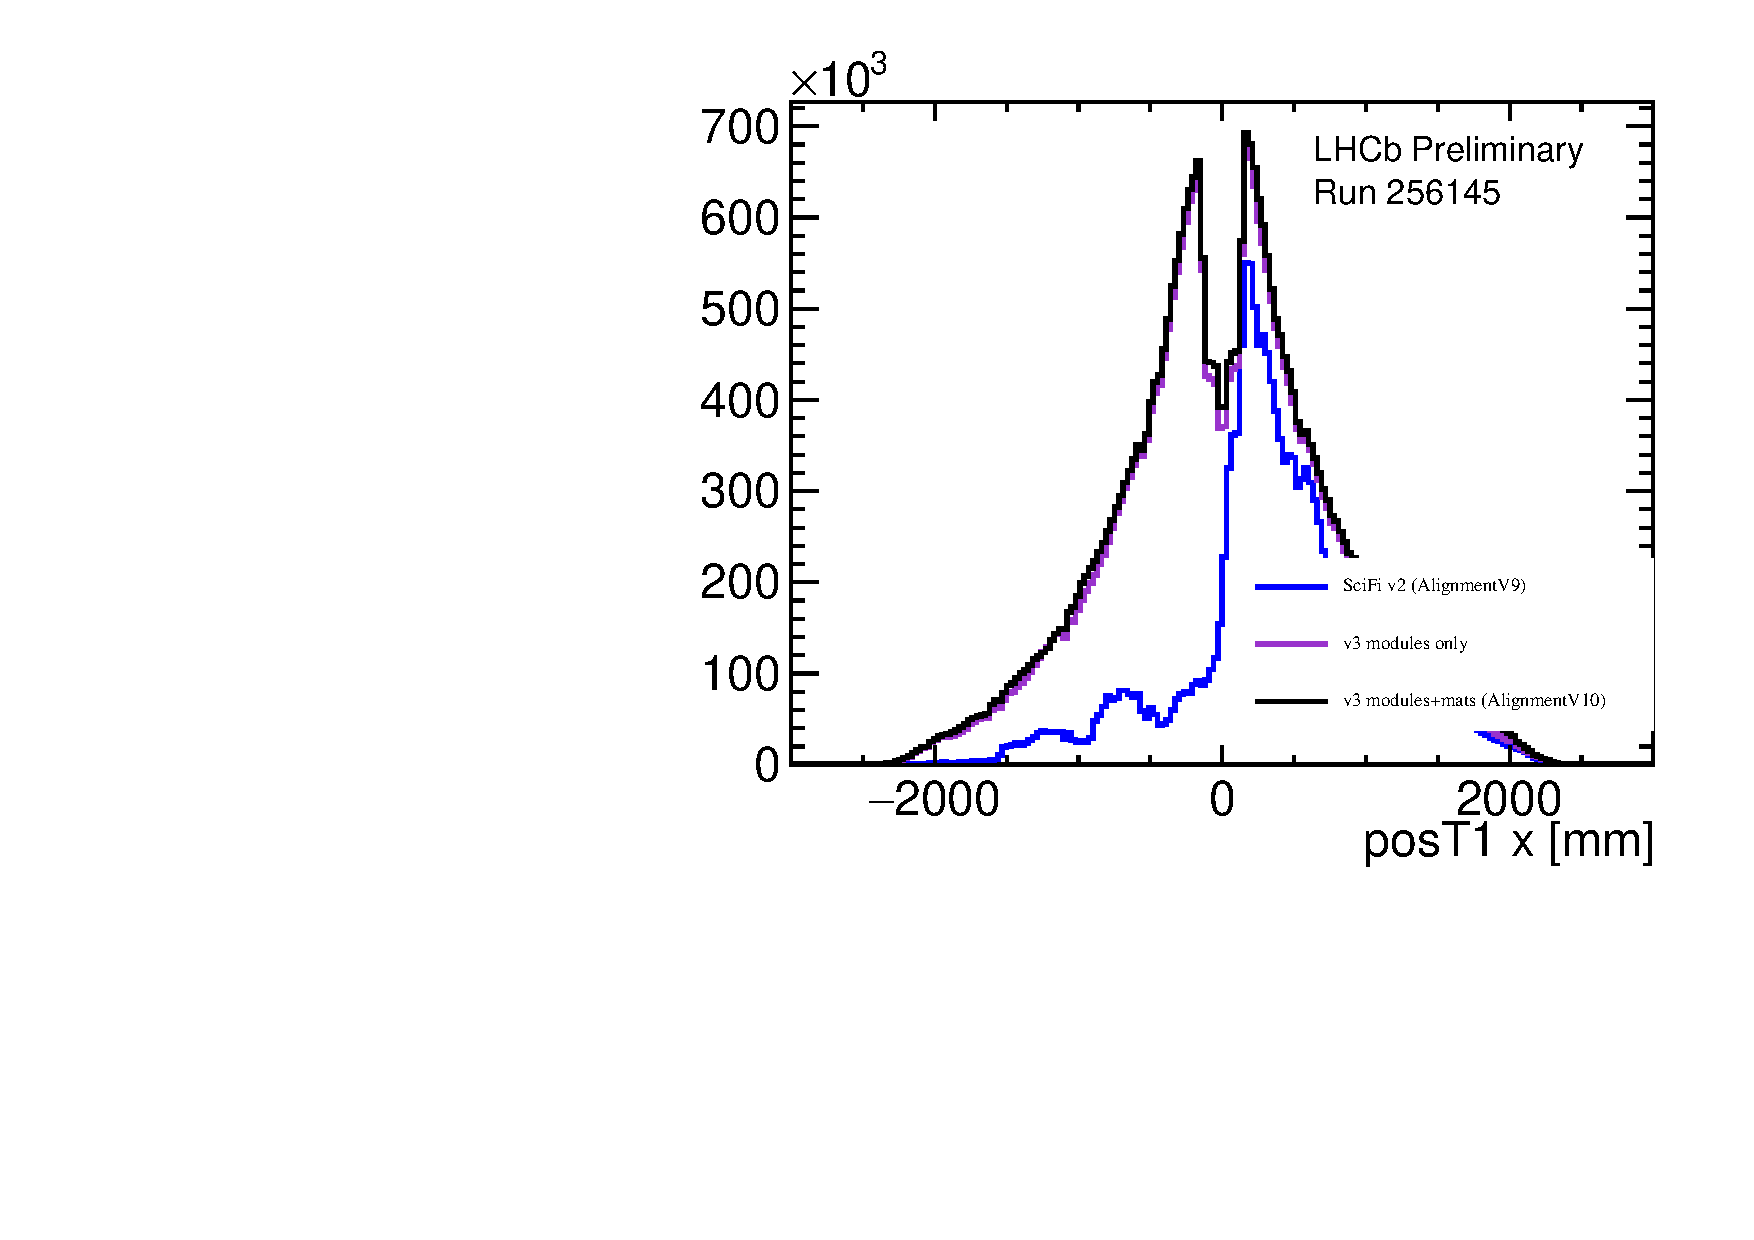
\includegraphics[width=\textwidth]{plots/xT1_moore.pdf}
      \end{figure}
    \end{column}
    \begin{column}[c]{0.49\textwidth}
      \begin{figure}
        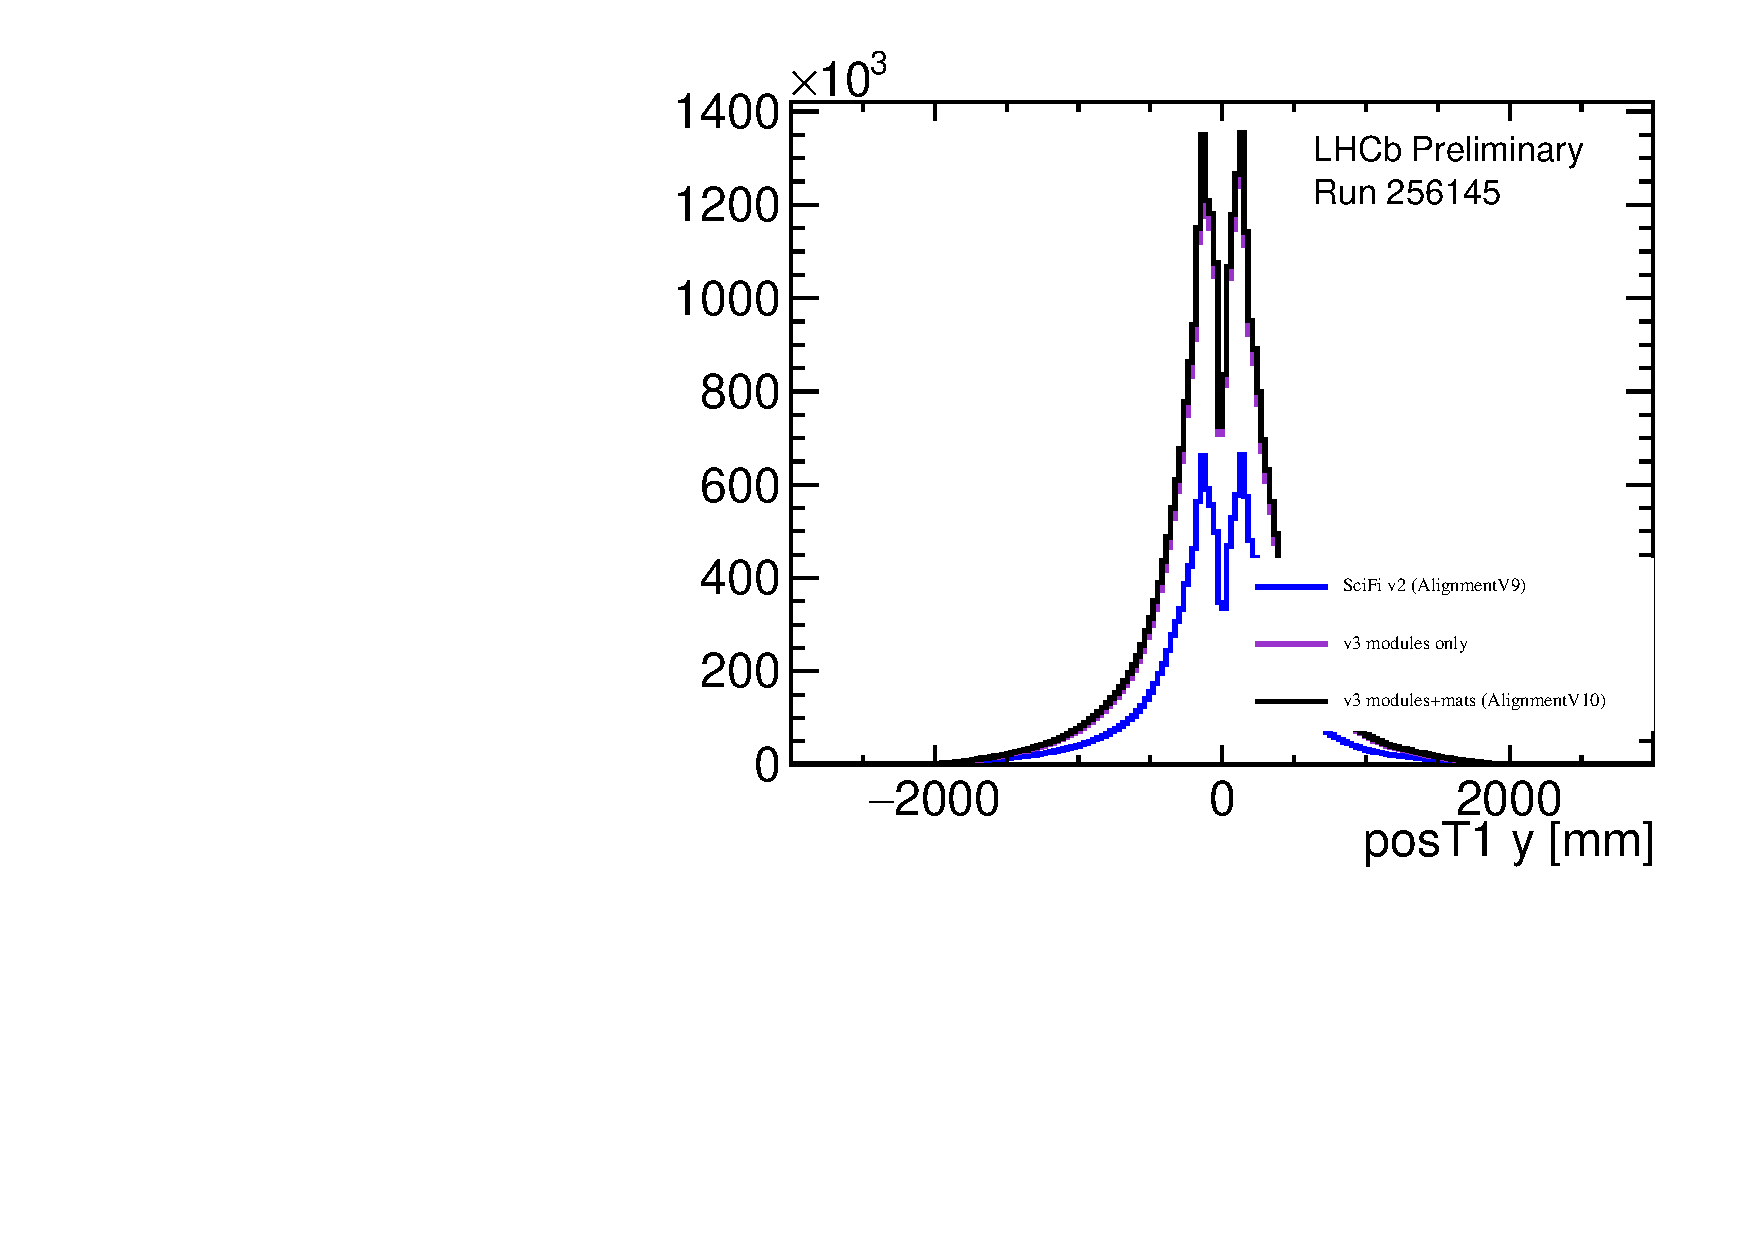
\includegraphics[width=\textwidth]{plots/yT1_moore.pdf}
      \end{figure}
    \end{column}
  \end{columns}  
\end{frame}

\begin{frame}\frametitle{Performance of v3 alignment on 2022 data}
  \begin{columns}
    \begin{column}[c]{0.49\textwidth}
      \begin{figure}
        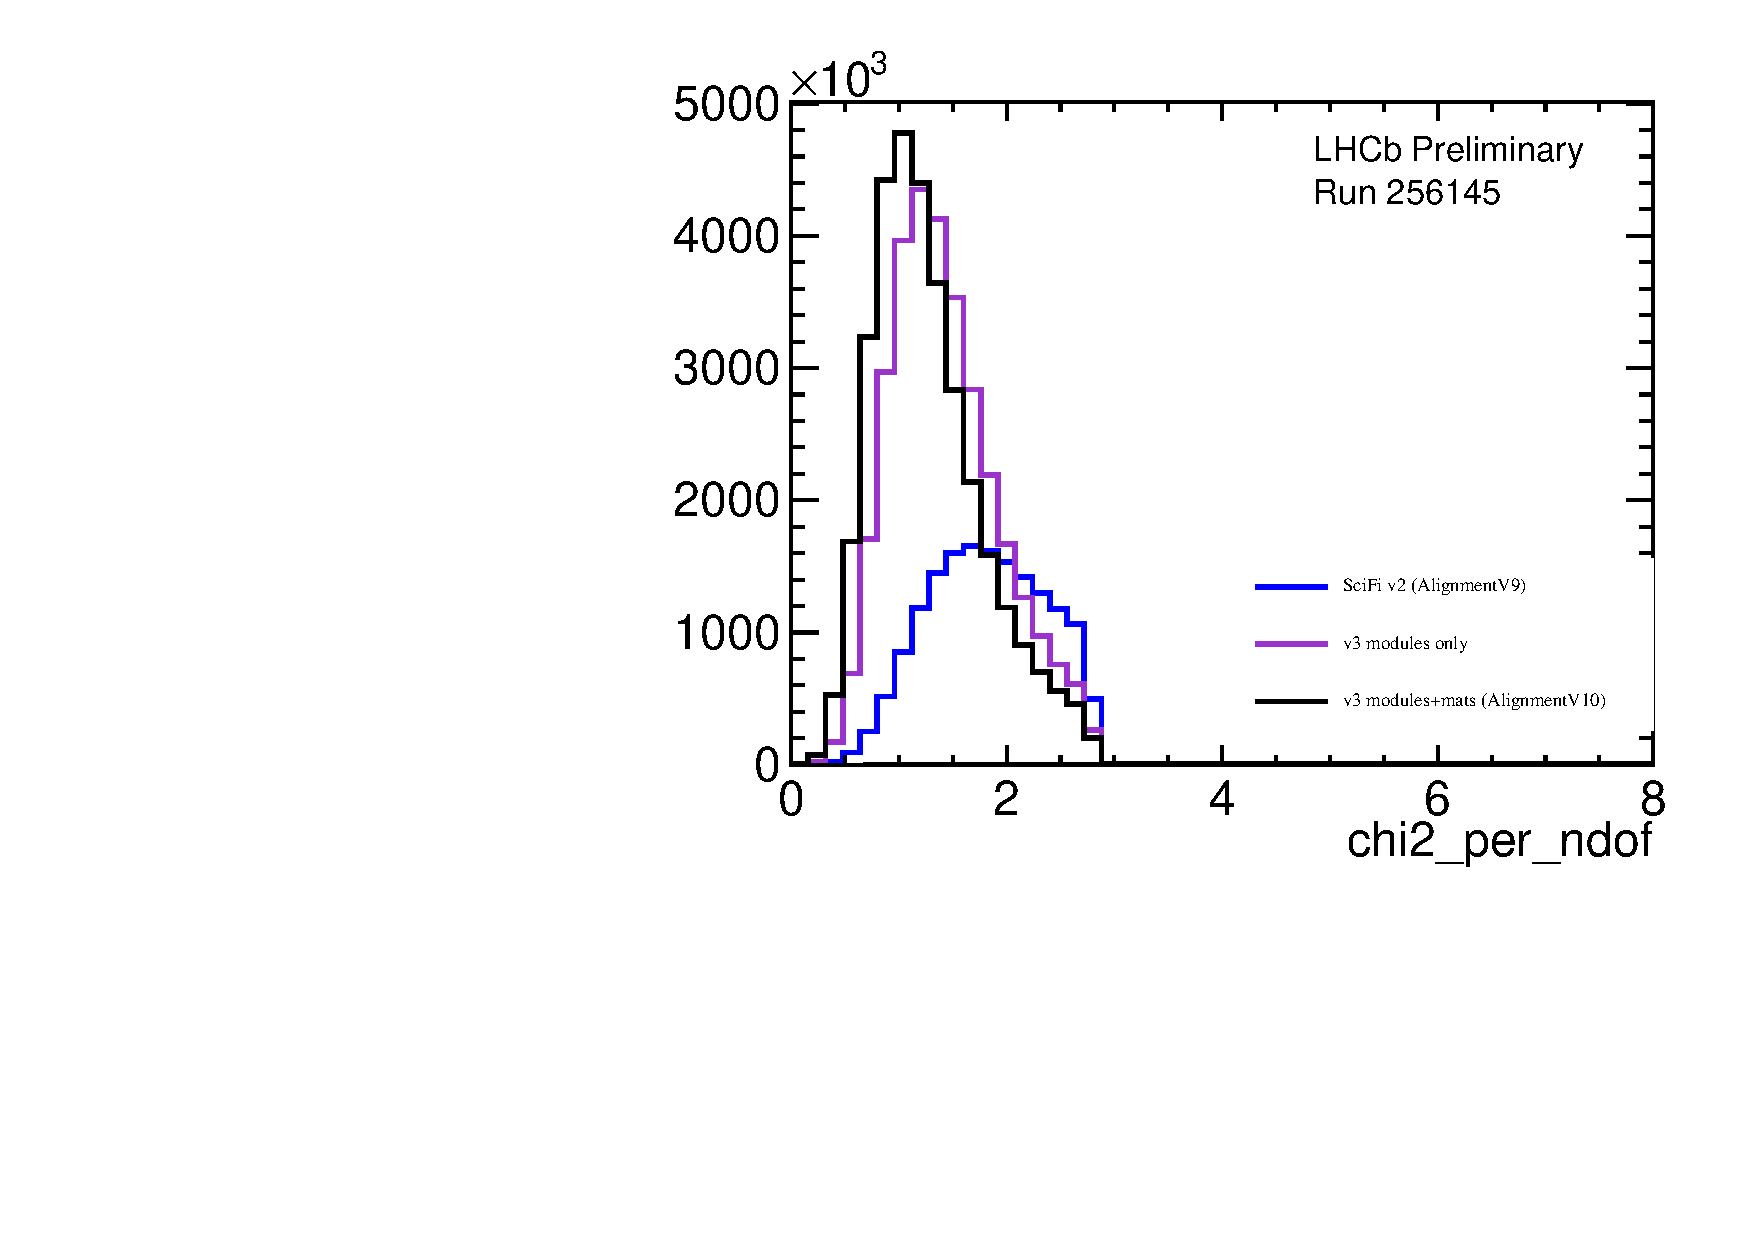
\includegraphics[width=\textwidth]{plots/chi2_moore.pdf}
      \end{figure}
    \end{column}
    \begin{column}[c]{0.49\textwidth}
      \begin{figure}
        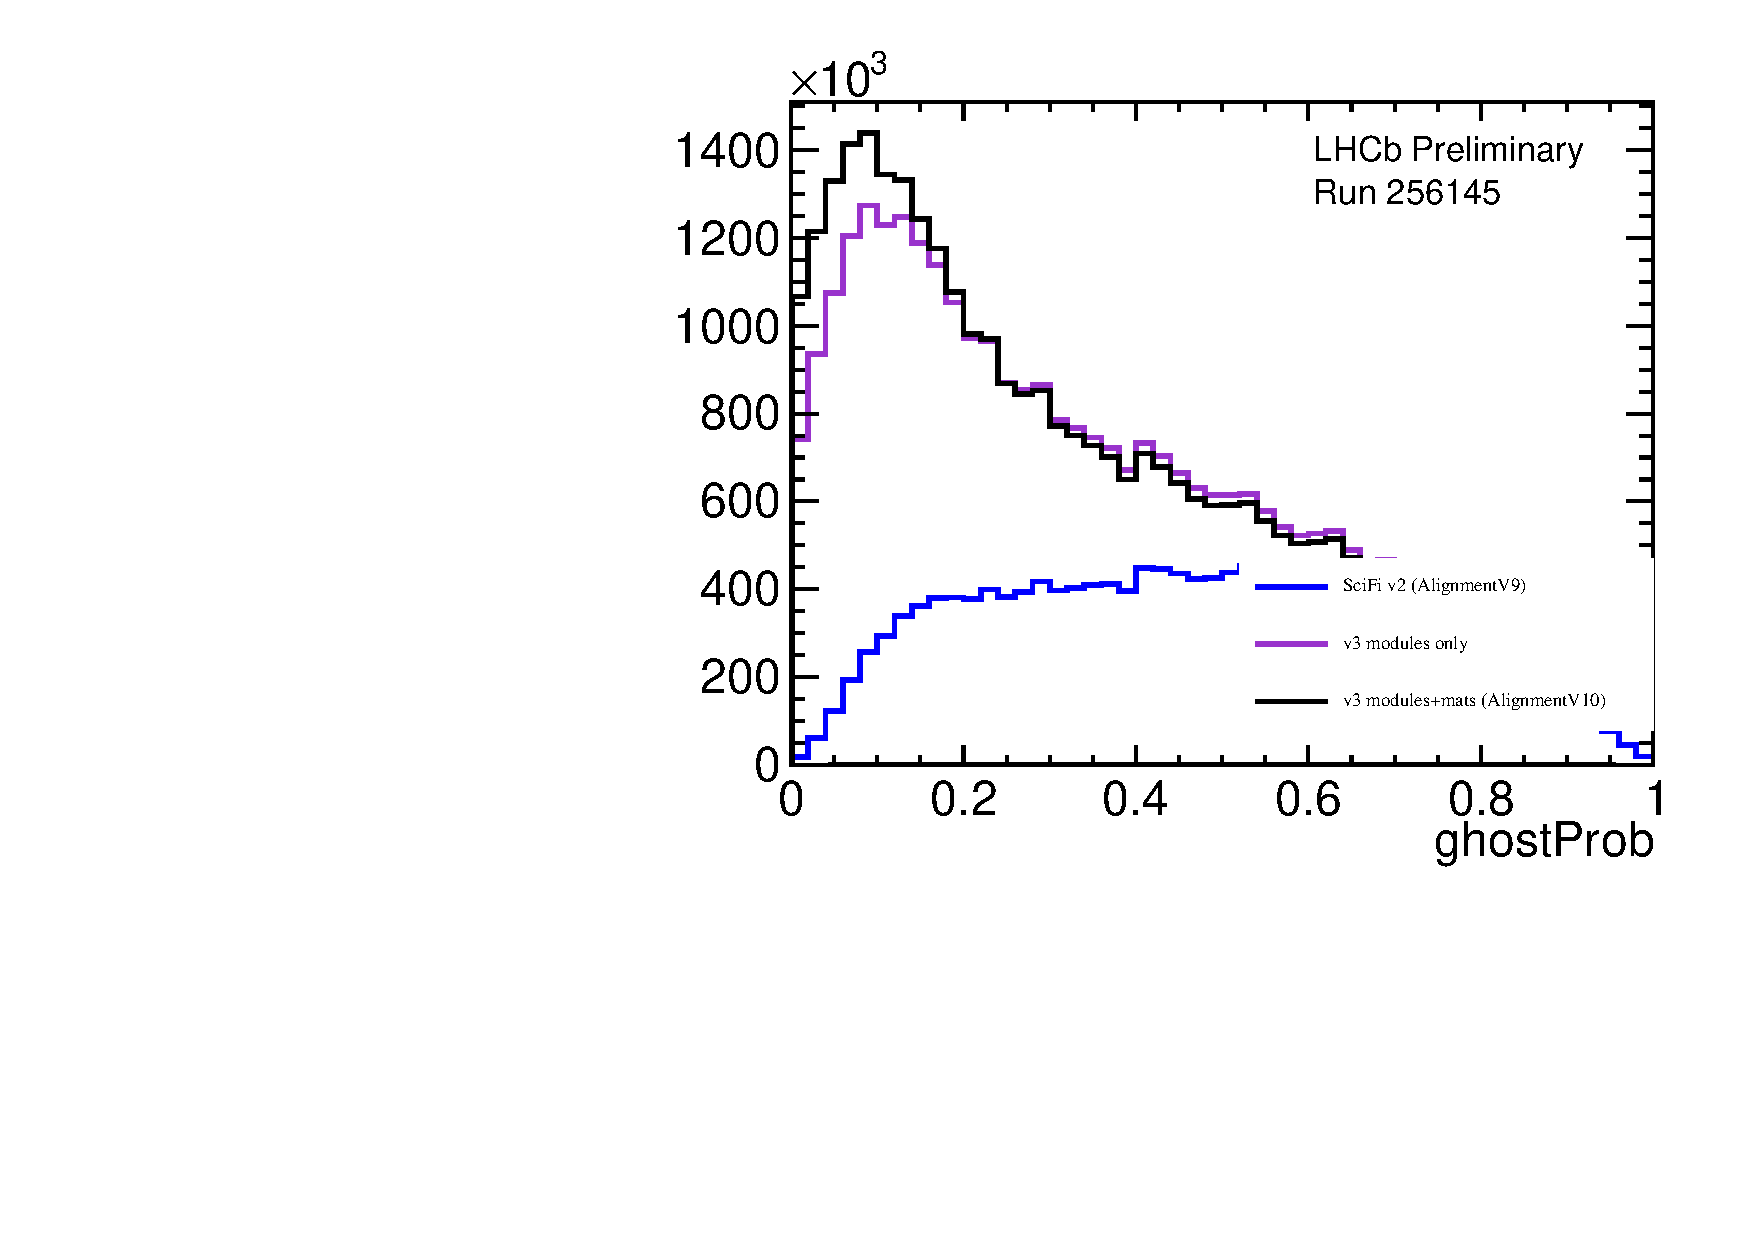
\includegraphics[width=\textwidth]{plots/ghost_moore.pdf}
      \end{figure}
    \end{column}
  \end{columns}  
\end{frame}

\begin{frame}\frametitle{Performance of v3 alignment on 2022 data}
  \begin{columns}
    \begin{column}[c]{0.49\textwidth}
      \begin{figure}
        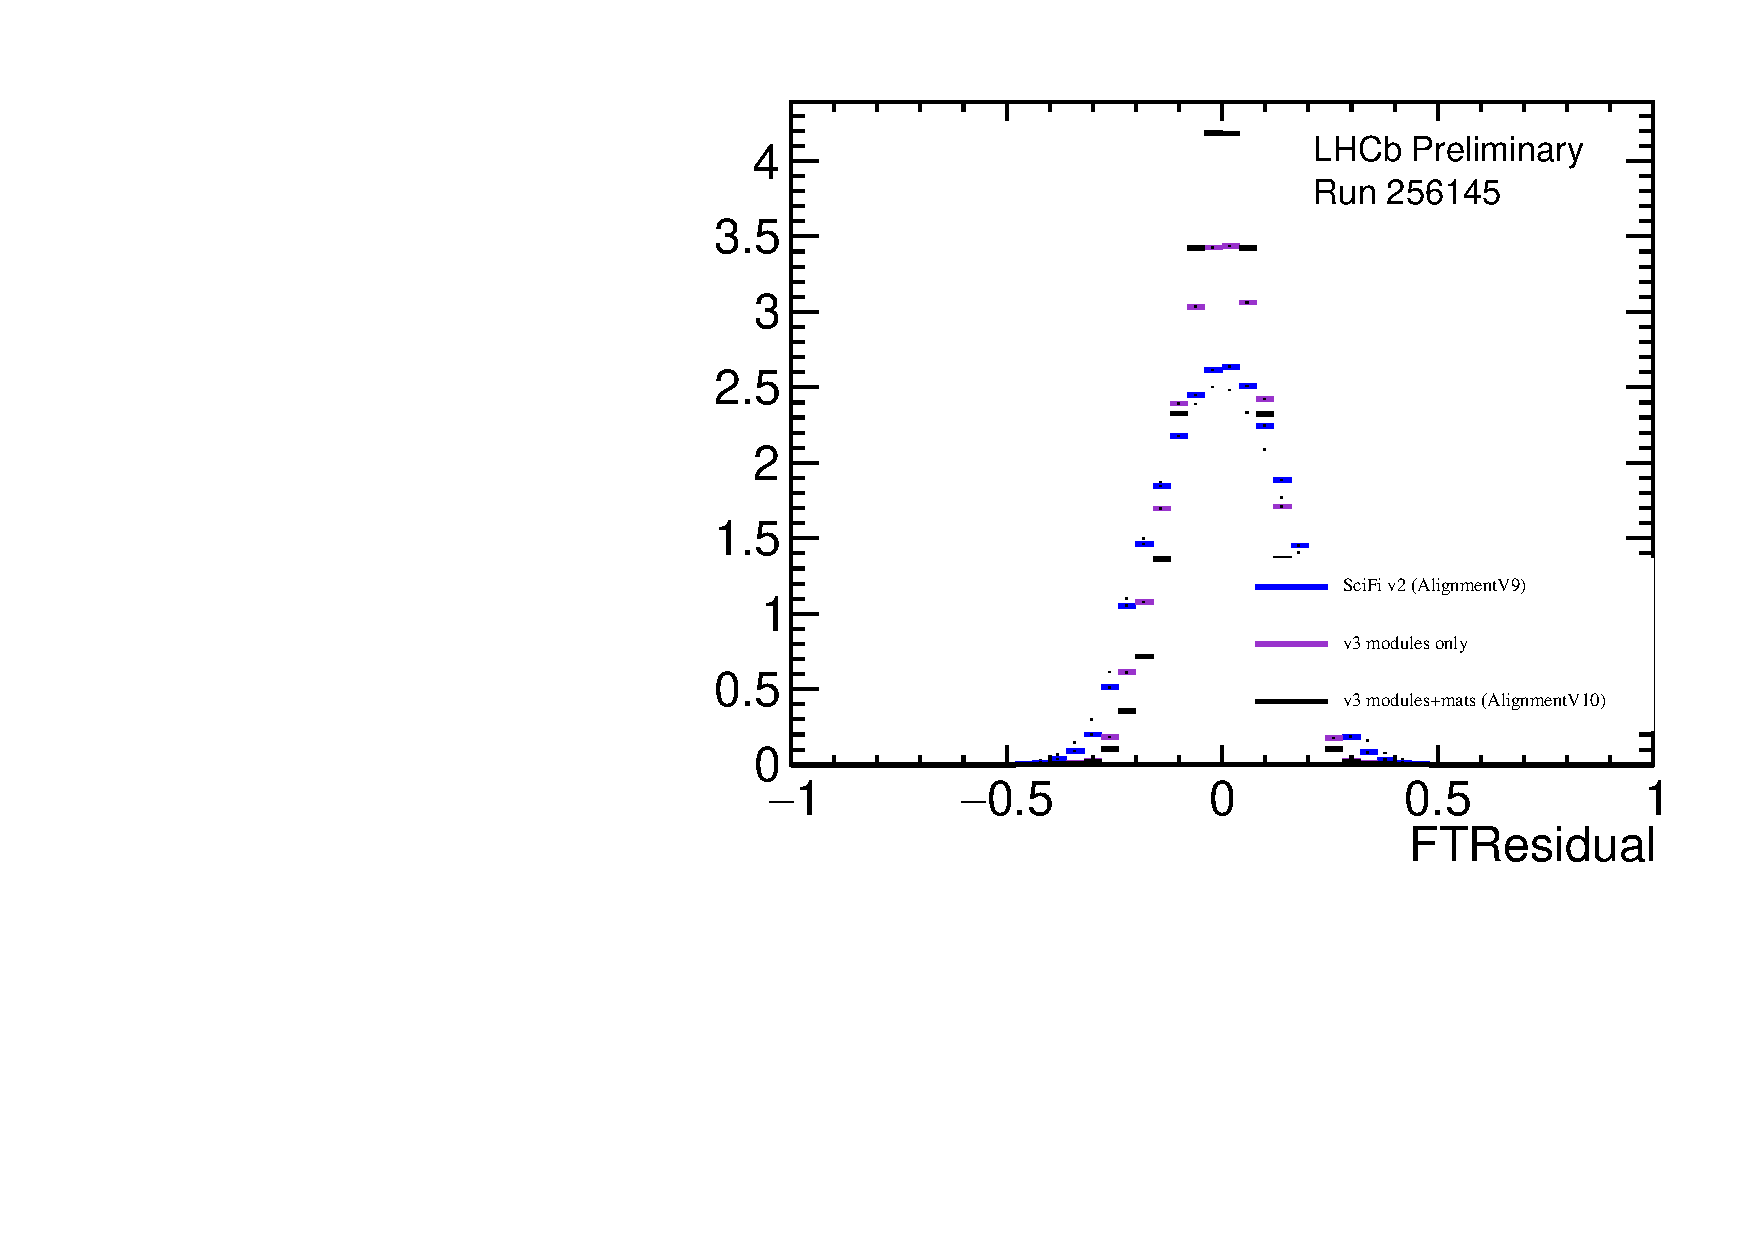
\includegraphics[width=0.7\textwidth]{plots/FTResidual_moore.pdf}
      \end{figure}
      Residual std. dev:
      \begin{itemize}
        \item - AlignmentV9: 0.137
        \item - v3 modules: 0.110
        \item - AlignmentV10: 0.096
      \end{itemize}
    \end{column}
    \begin{column}[c]{0.51\textwidth}
      \begin{figure}
        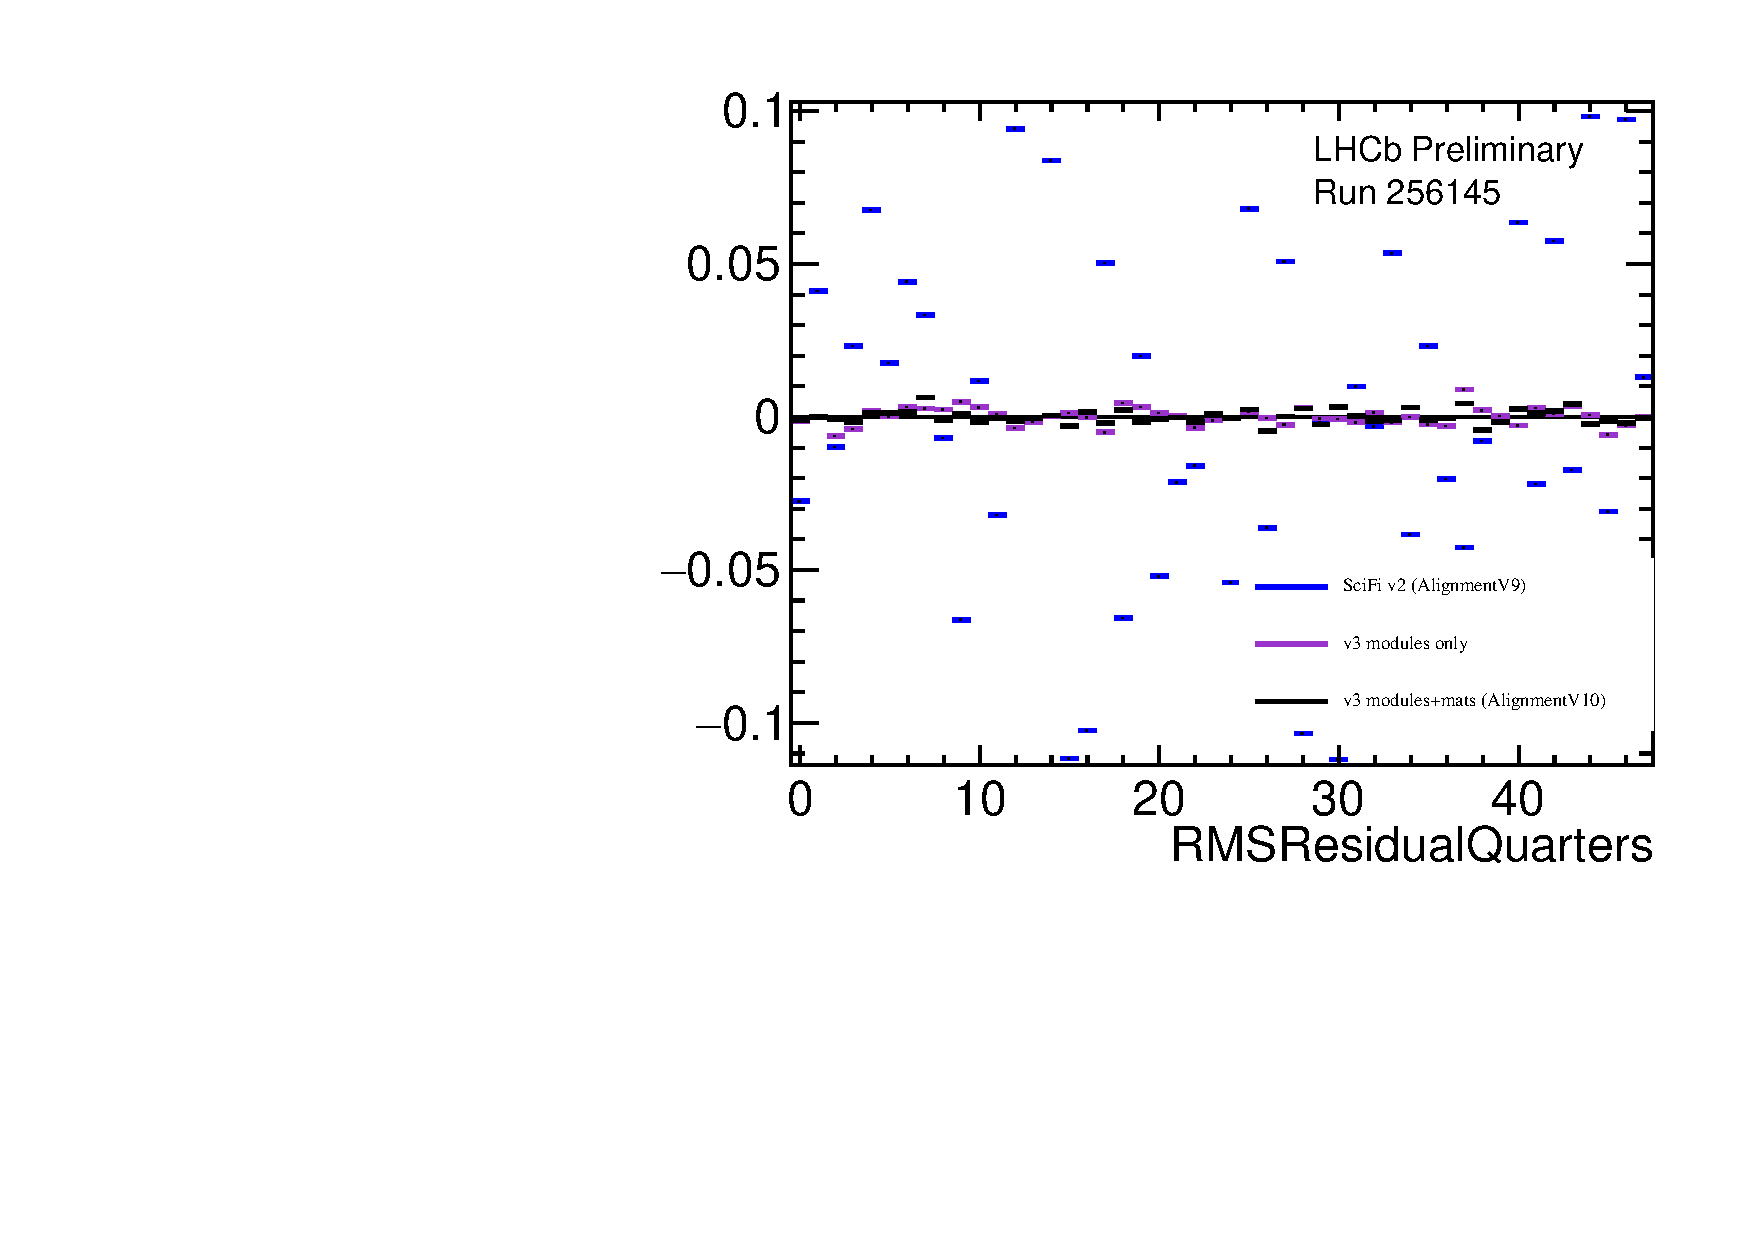
\includegraphics[width=\textwidth]{plots/RMSResidual_moore.pdf}
      \end{figure}
    \end{column}
  \end{columns}  
\end{frame}

\begin{frame}\frametitle{$\Lambda^0$ decays in different alignment versions}
  \begin{columns}
    \begin{column}[c]{0.49\textwidth}
      \begin{figure}
        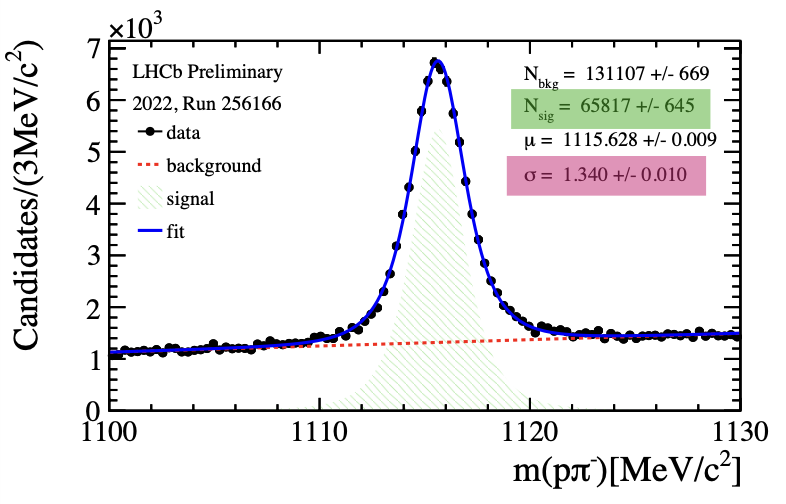
\includegraphics[width=0.9\textwidth]{plots/v9_lambda.png}
      \end{figure}
    \end{column}
    \begin{column}[c]{0.49\textwidth}
      \begin{itemize}
        \item Candidates: $\symbf{\symup{\Lambda_0}} \to\, \symup{p} \pi^{-}$/$\overline{\symbf{\symup{\Lambda_0}}} \to\, \overline{\symup{p}} \pi{+}$
        \item Huge improvements in signal yields (x2 from v9 to v10)
        \item Slightly improve mass peak resolution
        \item \href{https://indico.cern.ch/event/1275407/contributions/5419773/attachments/2653633/4595138/LC_WP4_5_250523.pdf}{Lukas' slides} % link his slides from P4/5 presentation
      \end{itemize}
      \begin{figure}
        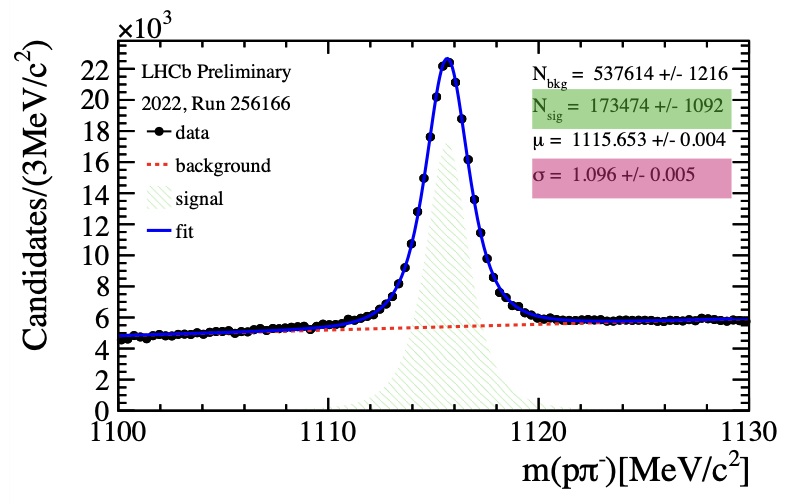
\includegraphics[width=0.9\textwidth]{plots/v10_lambda.png}
      \end{figure}
    \end{column}
  \end{columns}
\end{frame}

\begin{frame}\frametitle{$\Lambda^0$ decays: SciFi hits per track on s-weighted data}
  \begin{columns}
    \begin{column}[c]{0.48\textwidth}
      \begin{figure}
        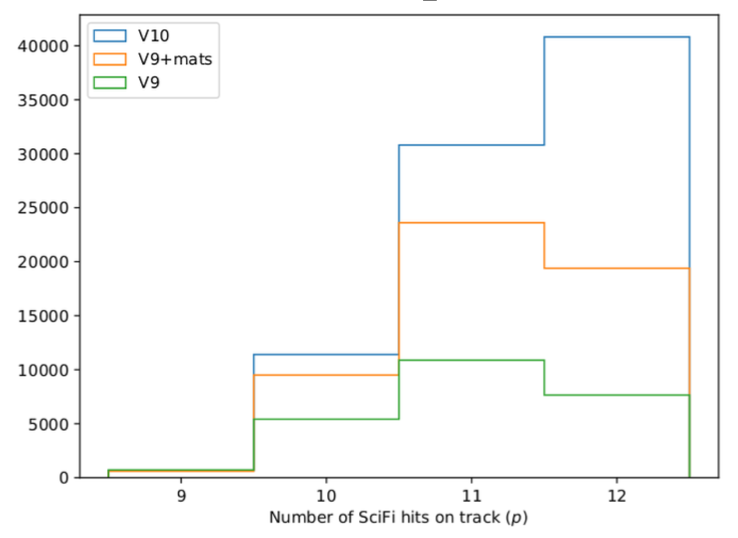
\includegraphics[width=0.5\textwidth]{plots/pos_lambda.png}
        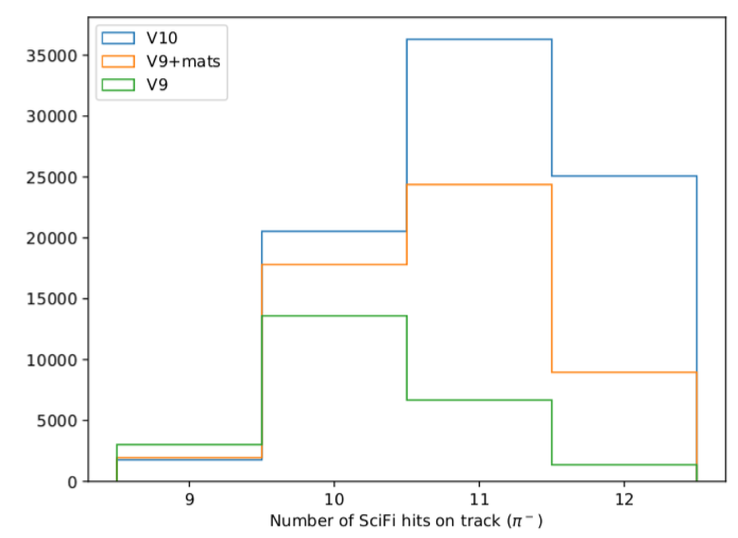
\includegraphics[width=0.5\textwidth]{plots/neg_lambda.png}
      \end{figure}
      \href{https://indico.cern.ch/event/1275407/contributions/5419773/attachments/2653633/4595138/LC_WP4_5_250523.pdf}{Lukas' slides} % link to lukas slides
    \end{column}
    \begin{column}[c]{0.48\textwidth}
      \begin{itemize}
        \item - Huge improvement on reconstructed tracks with 10, 11, 12 hits
        \item - Significantly higher average number of SciFi hits on tracks from version to version
        \item - We also see a significant charge asymmetry in $\Lambda$ decays
      \end{itemize}
      \begin{figure}
        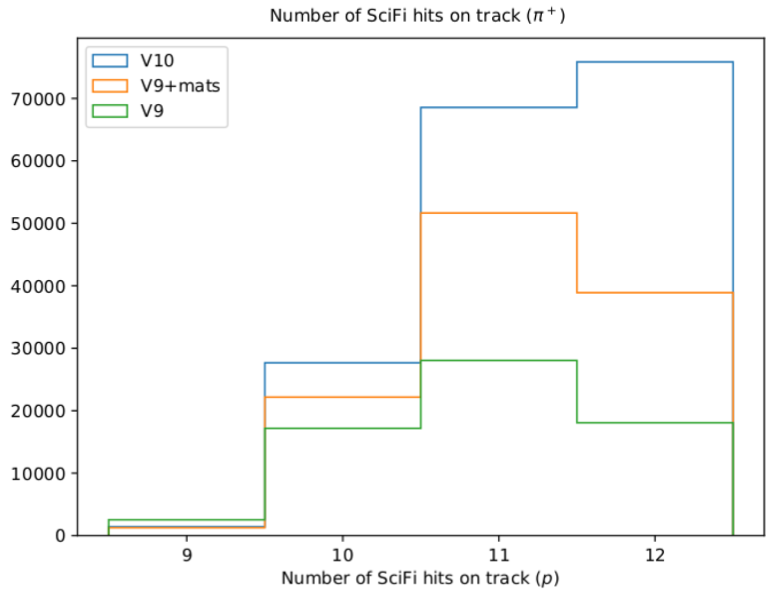
\includegraphics[width=0.5\textwidth]{plots/sw_lambda.png}
      \end{figure}
    \end{column}
  \end{columns}
\end{frame}

\begin{frame}\frametitle{Stability cross check on 2022 data}
  \begin{columns}
    \begin{column}[c]{0.48\textwidth}
      \begin{itemize}
	      \item $\bullet$\, Showing translation in x vs module number
	      \item $\bullet$\, MD run comparison
	      \item $\bullet$\, runs from same fill yield consistent results
	      \item $\bullet$\, run 256030 without fine timing worse as expected \to\, newer runs clearly better!
	      \item $\bullet$\, Most translations are within 1 mm which is expected from survey measurements
      \end{itemize}
    \end{column}
    \begin{column}[c]{0.48\textwidth}
      Exemplary plot for T3X2
      \begin{figure}
      	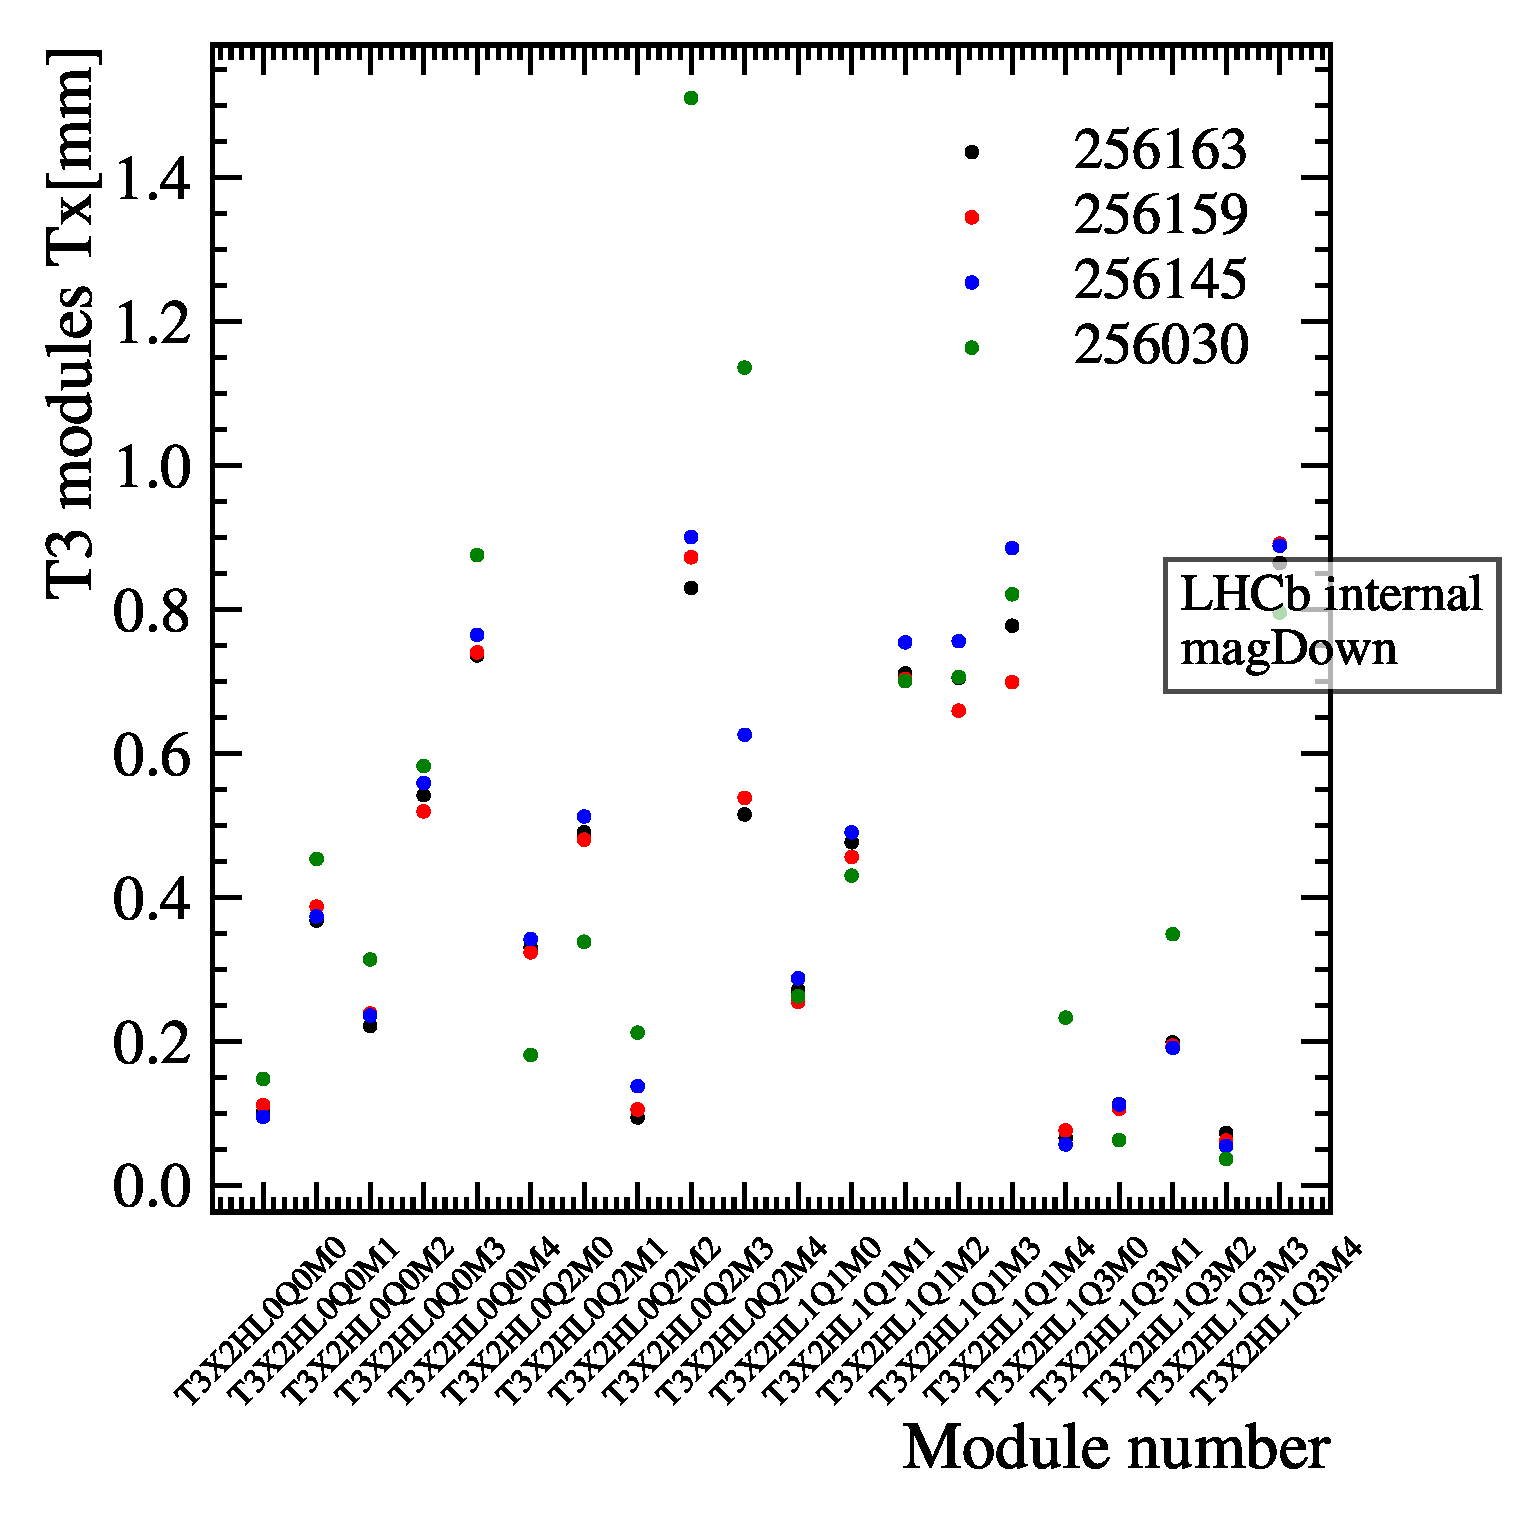
\includegraphics[width=0.9\textwidth]{positions_study_yamls/2023-05-31/outfiles/T3X2_Tx_constrain.pdf}
      \end{figure}
    \end{column}
  \end{columns}
\end{frame}

\begin{frame}\frametitle{Survey and Photogrammetry for 2023}
  \begin{columns}
    \begin{column}[c]{0.52\textwidth}
      \begin{figure}
        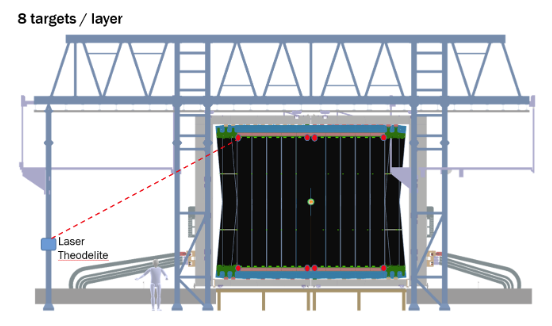
\includegraphics[width=\textwidth]{plots/survey_photo.png}
      \end{figure}
      Big thanks to Maria, Blake, Pascal S, Rodolphe and the whole survey team!
    \end{column}
    \begin{column}[c]{0.48\textwidth}
      \begin{itemize}
        \item $\bullet$\, Survey taken: feb 20th - march 9th
        \item $\bullet$\, 4 measurement points per C-frame at corners
        \item $\bullet$\, Target: keep inner modules as close to nominal as possible, outer edges can move as needed
        \item $\bullet$\, Summary: 450 microns in Z, most frames within 200 microns from nominal
        \item $\bullet$\, 400 microns in X, 1.5 mm in Y
        \item $\bullet$\, On average 400 - 600 microns in Y, 50 - 200 microns in the center region
      \end{itemize}
    \end{column}
  \end{columns}
\end{frame}

\begin{frame}\frametitle{Survey and Photogrammetry for 2023}
  \begin{columns}
    \begin{column}[c]{0.48\textwidth}
      \begin{figure}
        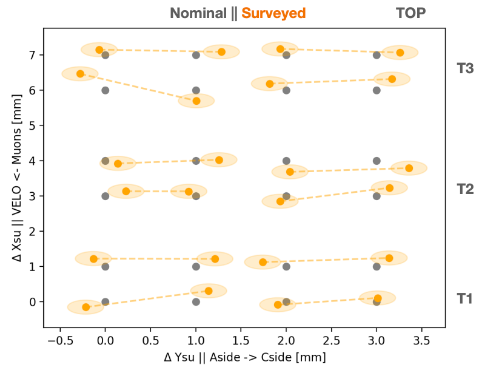
\includegraphics[width=0.9\textwidth]{plots/survey_top.png}
      \end{figure}
    \end{column}
    \begin{column}[c]{0.48\textwidth}
      \begin{figure}
        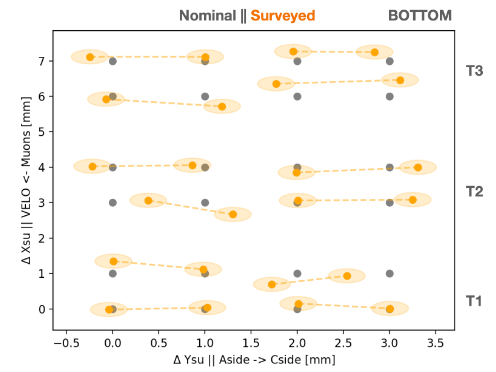
\includegraphics[width=0.9\textwidth]{plots/survey_bottom.png}
      \end{figure}
    \end{column}
  \end{columns}
  \begin{itemize}
    \item $\bullet$\, Top/bottom view of the respective edges $\pm \SI{2.5}{\m}$ above/below beam pipe
    \item $\bullet$\, $\SI{200}{\micro\m}$ survey uncertainty
%      \item $\bullet$\, A-side \to +x, C-side \to -x
    \item $\bullet$\, T1, T2: outer layers surveyed \to L0 and L3
%      \item $\bullet$\, L0 and L2 in every T-station since we can only view the front of the C-frame
  \end{itemize}
\end{frame}

\begin{frame}\frametitle{Survey and Photogrammetry for 2023}
  \begin{columns}
    \begin{column}[c]{0.48\textwidth}
      \begin{figure}
        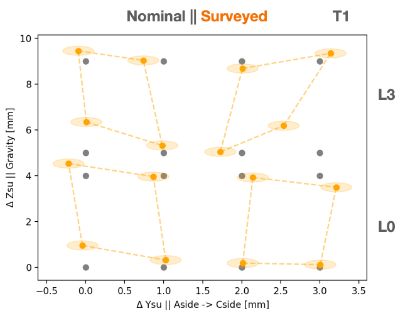
\includegraphics[width=0.6\textwidth]{plots/survey_T1.png}
        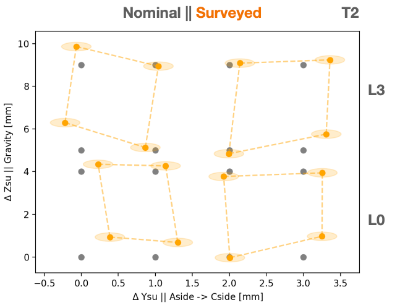
\includegraphics[width=0.6\textwidth]{plots/survey_T2.png}
      \end{figure}
    \end{column}
    \begin{column}[c]{0.48\textwidth}
      \begin{itemize}
        \item $\bullet$\, T3: L0 and L2 surveyed (L3 targets in RICH volume)
        \item $\bullet$\, T3L2 measured between L1 and L2 with smaller targets
        \item $\bullet$\, Possible movement during measurement
      \end{itemize}
      \begin{figure}
        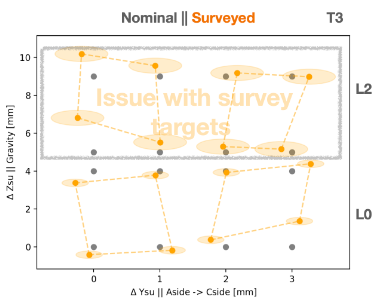
\includegraphics[width=0.6\textwidth]{plots/survey_T3.png}
      \end{figure}
    \end{column}
  \end{columns}
\end{frame}

\begin{frame}\frametitle{Readout Map adaptations}
  \begin{columns}
    \begin{column}[c]{0.52\textwidth}
      \begin{figure}
        
\includegraphics[width=\textwidth]{plots/merged_4096.png} \\
        \vspace{0.6cm}
        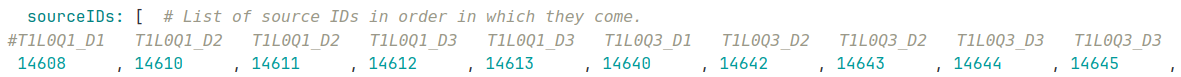
\includegraphics[width=\textwidth]{plots/old_readout.png} \\
        \vspace{0.6cm}
        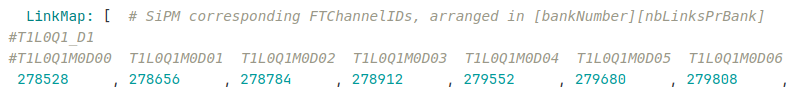
\includegraphics[width=\textwidth]{plots/new_readout.png} \\
      \end{figure}
      Big thanks to Louis!
    \end{column}
    \begin{column}[c]{0.48\textwidth}
      \begin{itemize}
        \item $\bullet$\, Readout map \to\, Cabling Map
        \item $\bullet$\, Automatic fetching of deactivated links
        \item \to\, Deactivate links without changing readout map!
        \item $\bullet$\, 2022: no active link map 
        \item $\bullet$\, \to empty events
        \item $\bullet$\, \href{https://gitlab.cern.ch/lhcb/LHCb/-/merge_requests/4129}{LHCb!4129} improved flexibility
        \item $\bullet$\, 2023: allows to ignore dynamic link deactivation if no active link found
      \end{itemize}
    \end{column}
  \end{columns}
\end{frame}

\begin{frame}\frametitle{SciFi online alignment}
  \begin{columns}
    \begin{column}[c]{0.58\textwidth}
      \begin{figure}
	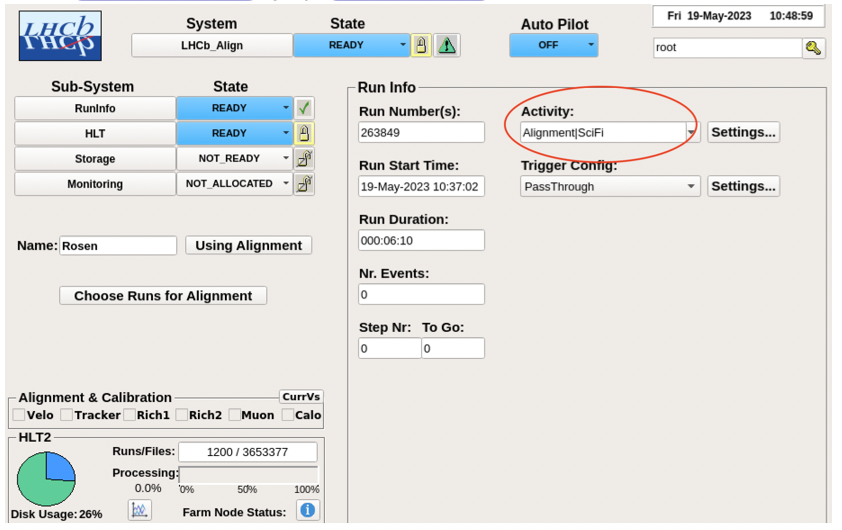
\includegraphics[width=\textwidth]{plots/align_run_control.png}
      \end{figure}
    \end{column}
    \begin{column}[c]{0.38\textwidth}
      \begin{itemize}
        \item \scriptsize $\bullet$\, SciFi alignment was added in the run control \href{https://gitlab.cern.ch/lhcb/MooreOnline/-/merge_requests/232}{MooreOnline!232} and \href{https://gitlab.cern.ch/lhcb/Alignment/-/merge_requests/378}{Alignment!378}
	      \item $\bullet$\, Detector elements and alignment adapted for DD4Hep: \href{https://gitlab.cern.ch/lhcb/Detector/-/merge_requests/363}{Detector!363} and \href{https://gitlab.cern.ch/lhcb/Alignment/-/merge_requests/364}{Alignment!364}
	      \item $\bullet$\, Next is to work on the online monitoring and estimate thresholds for automatic update while data taking
	      \item $\bullet$\, runs with recent mu scans (from 2023) used for evaluating the SciFi half modules alignment: Run 264400 : mu 6,71
      \end{itemize}
    \end{column}
  \end{columns}
\end{frame}

\begin{frame}\frametitle{SciFi alignment with 2023 data}
  \begin{columns}
    \begin{column}[c]{0.49\textwidth}
      \begin{itemize}
        \item \small $\bullet$\, Several configurations ran aligning the HalfModules: TxRxRz + average Tz constraint
        \item $\bullet$\, Translations in x within 1mm
      \end{itemize}
      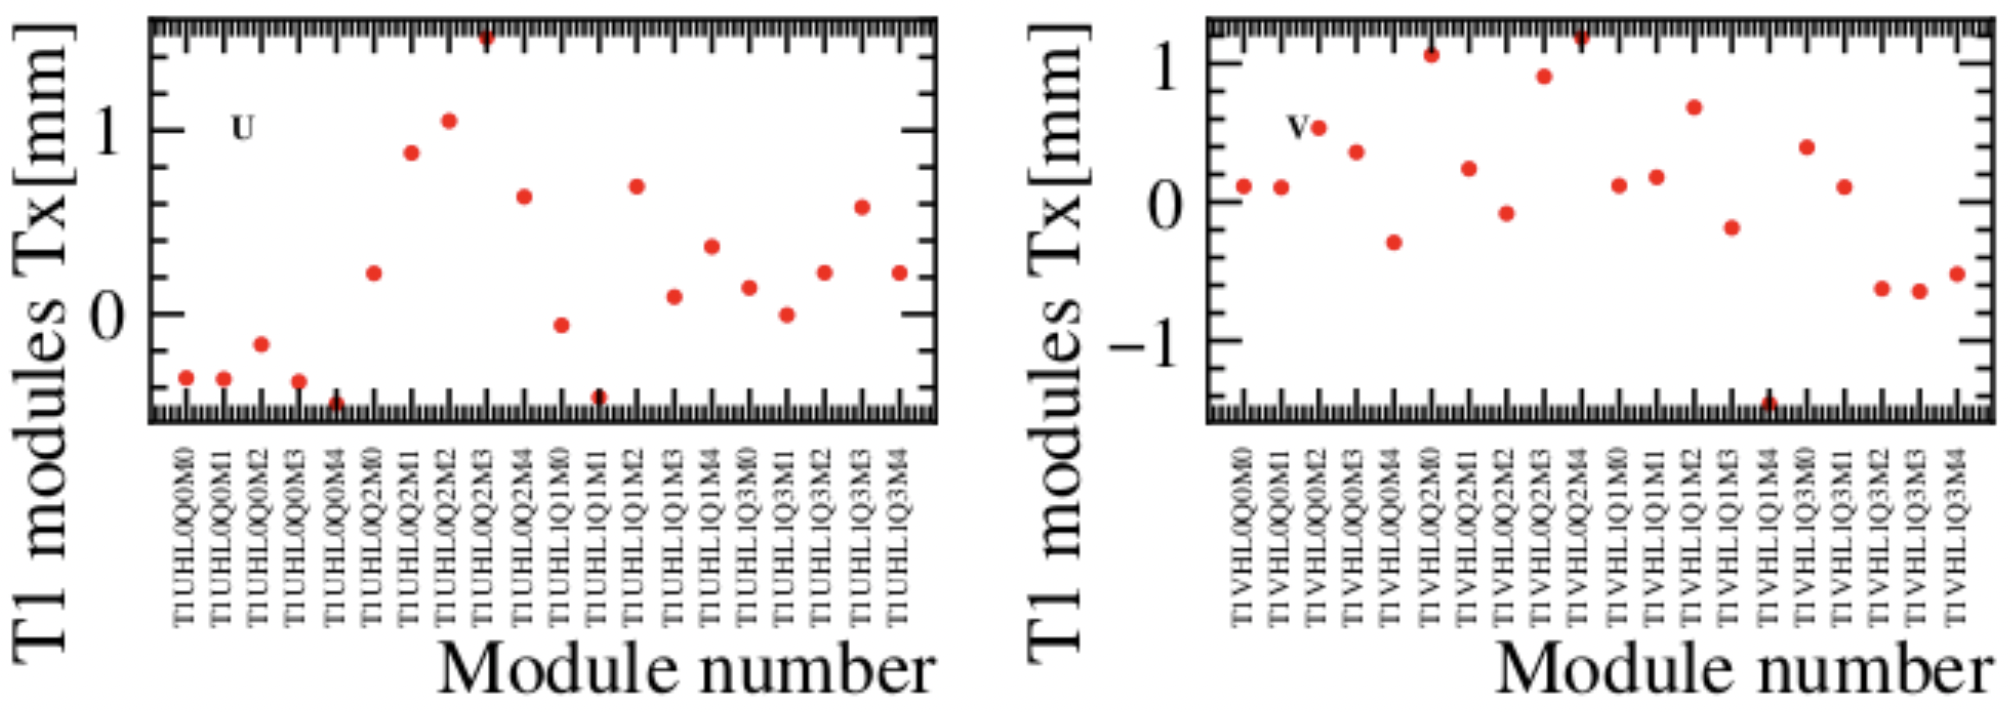
\includegraphics[width=0.6\textwidth]{plots/t1tx.png}
      \begin{itemize}
        \item $\bullet$\,Rotations in x within 1 mrad
      \end{itemize}
      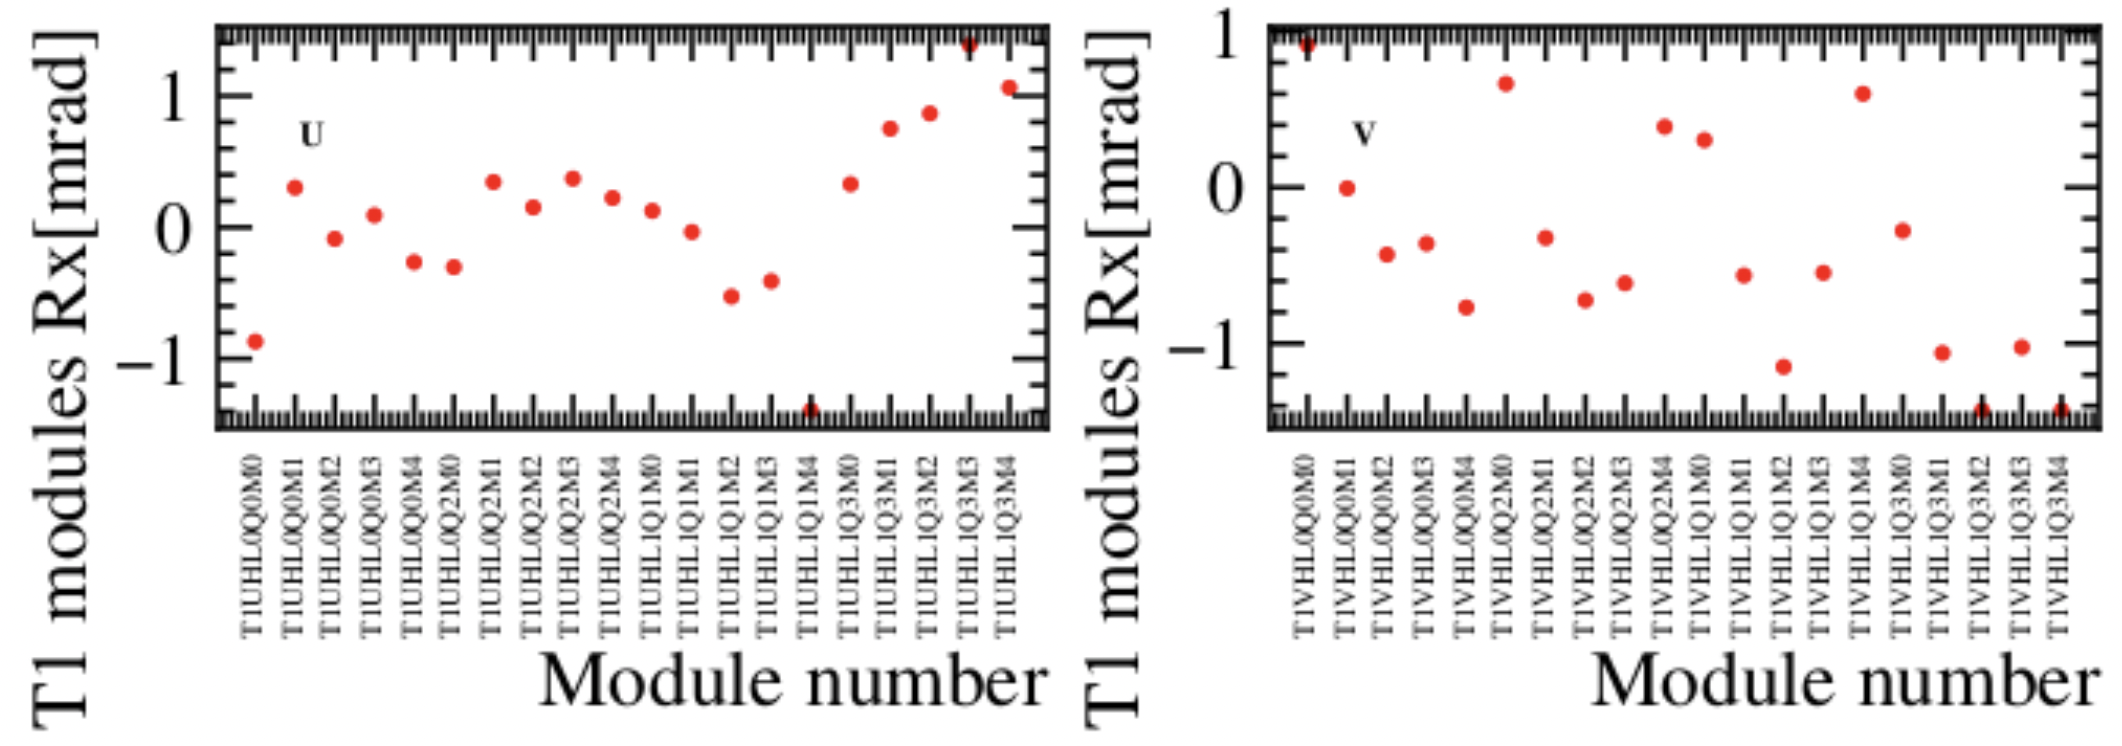
\includegraphics[width=0.6\textwidth]{plots/t1rx.png}
      \begin{itemize}
        \item $\bullet$\, New version of the module alignment (v5) was created based on this configuration
      \end{itemize}
    \end{column}
    \begin{column}[c]{0.49\textwidth}
      \begin{figure}
        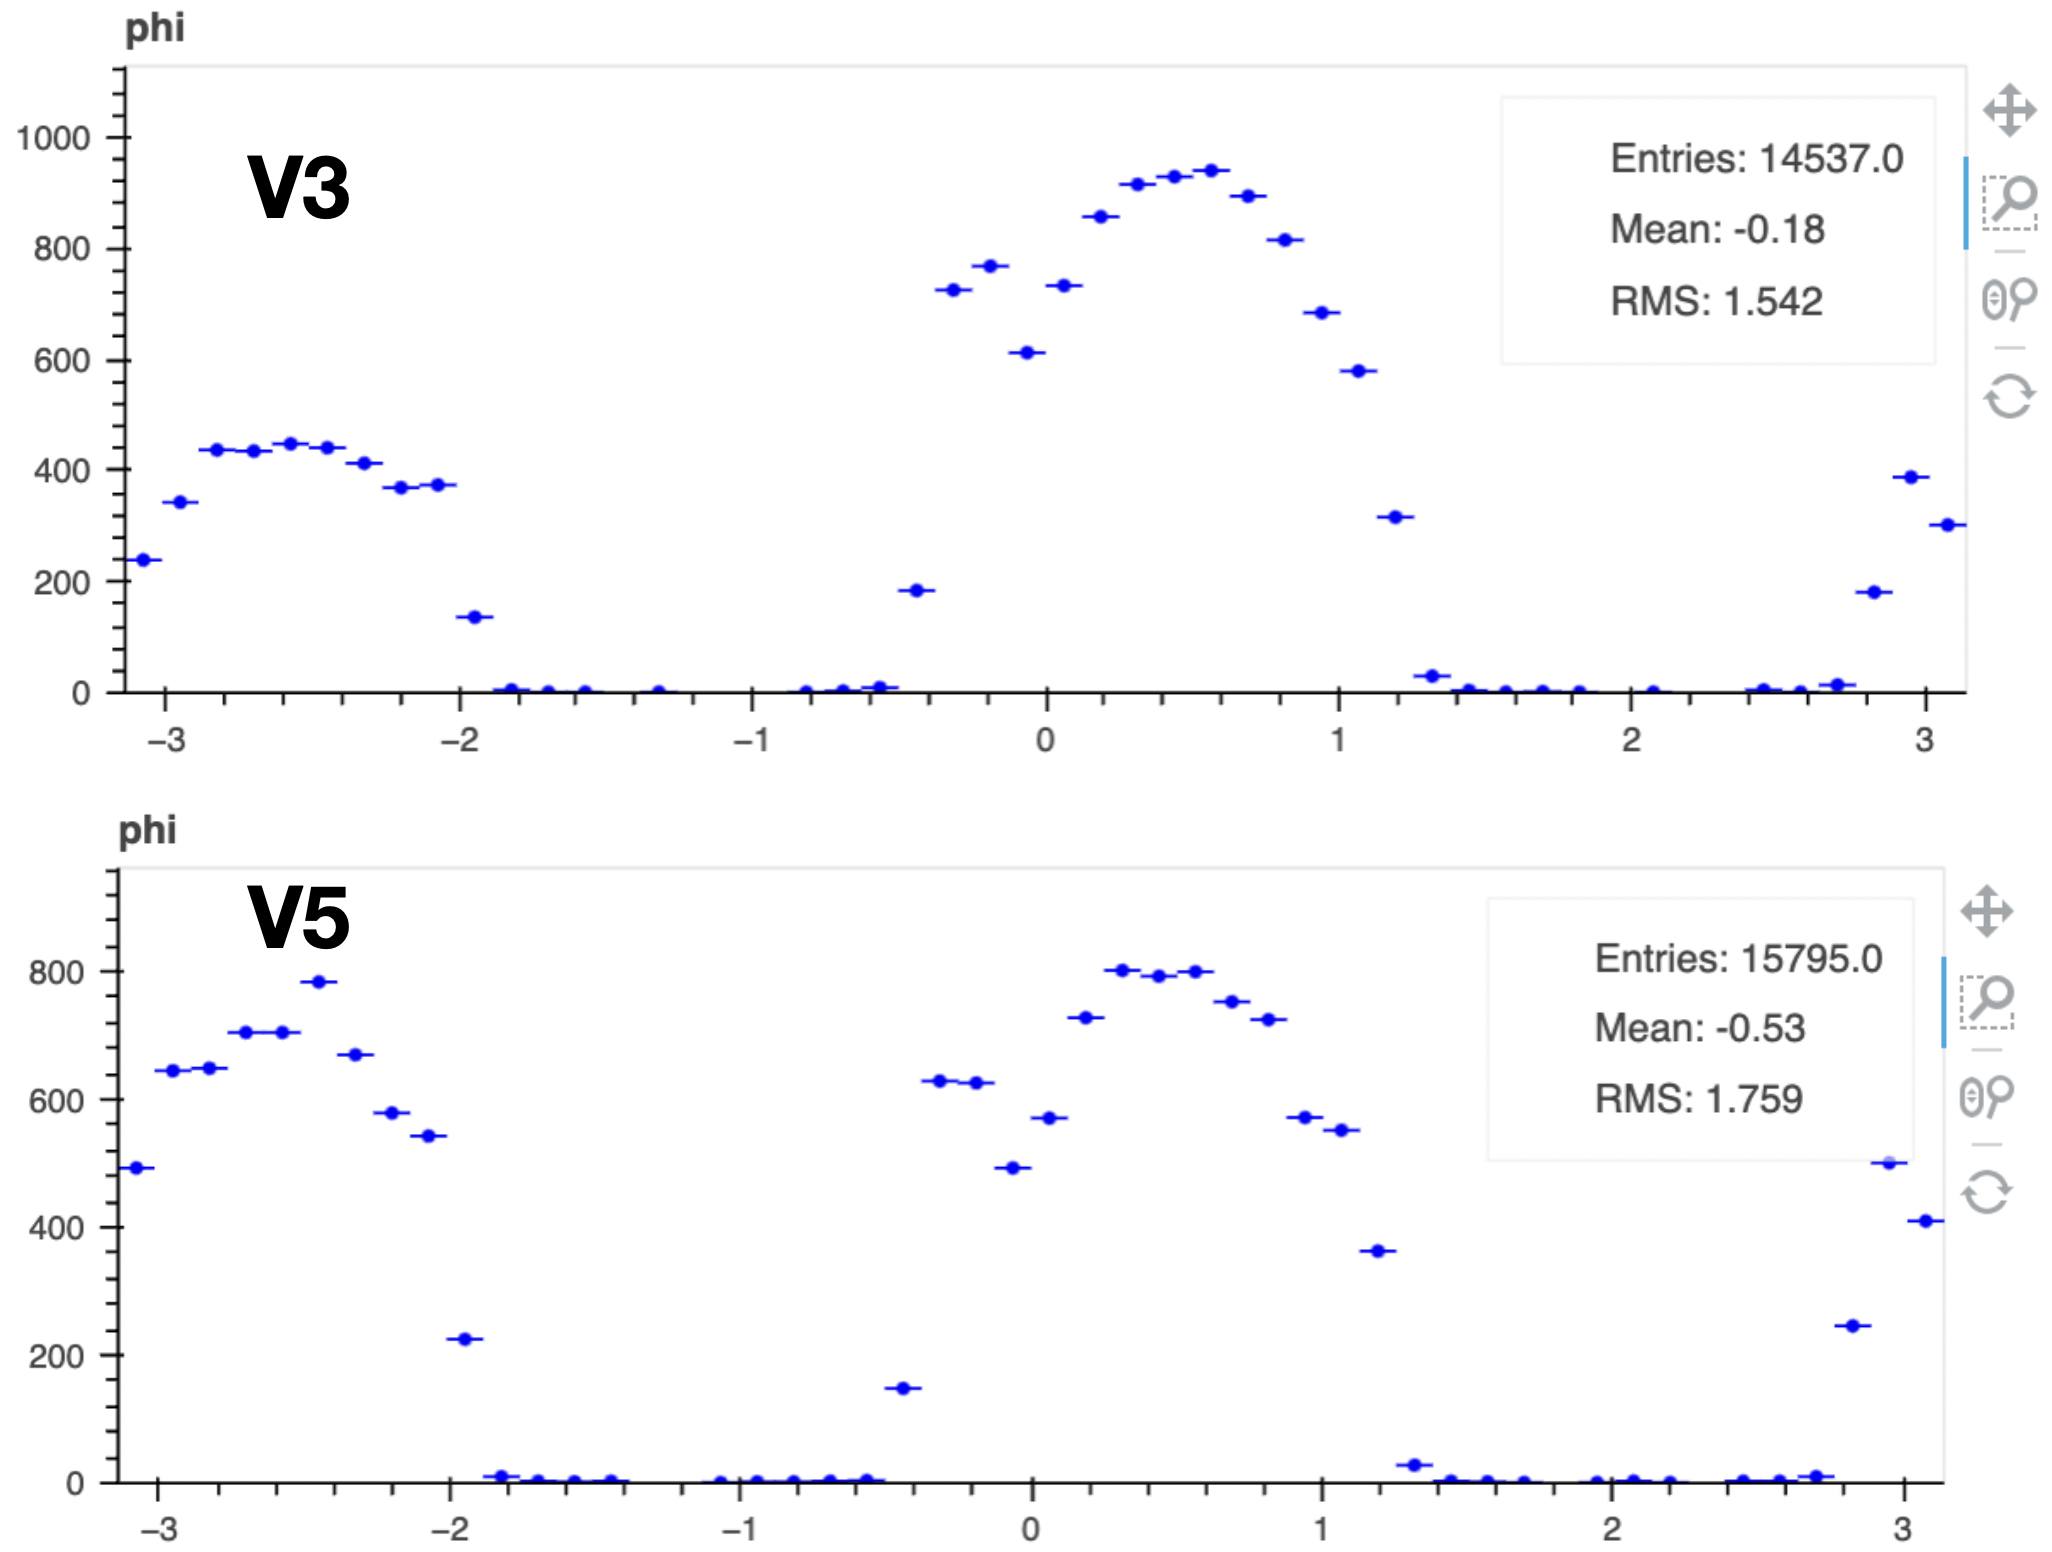
\includegraphics[width=0.5\textwidth]{plots/phi_v3v5.png}
        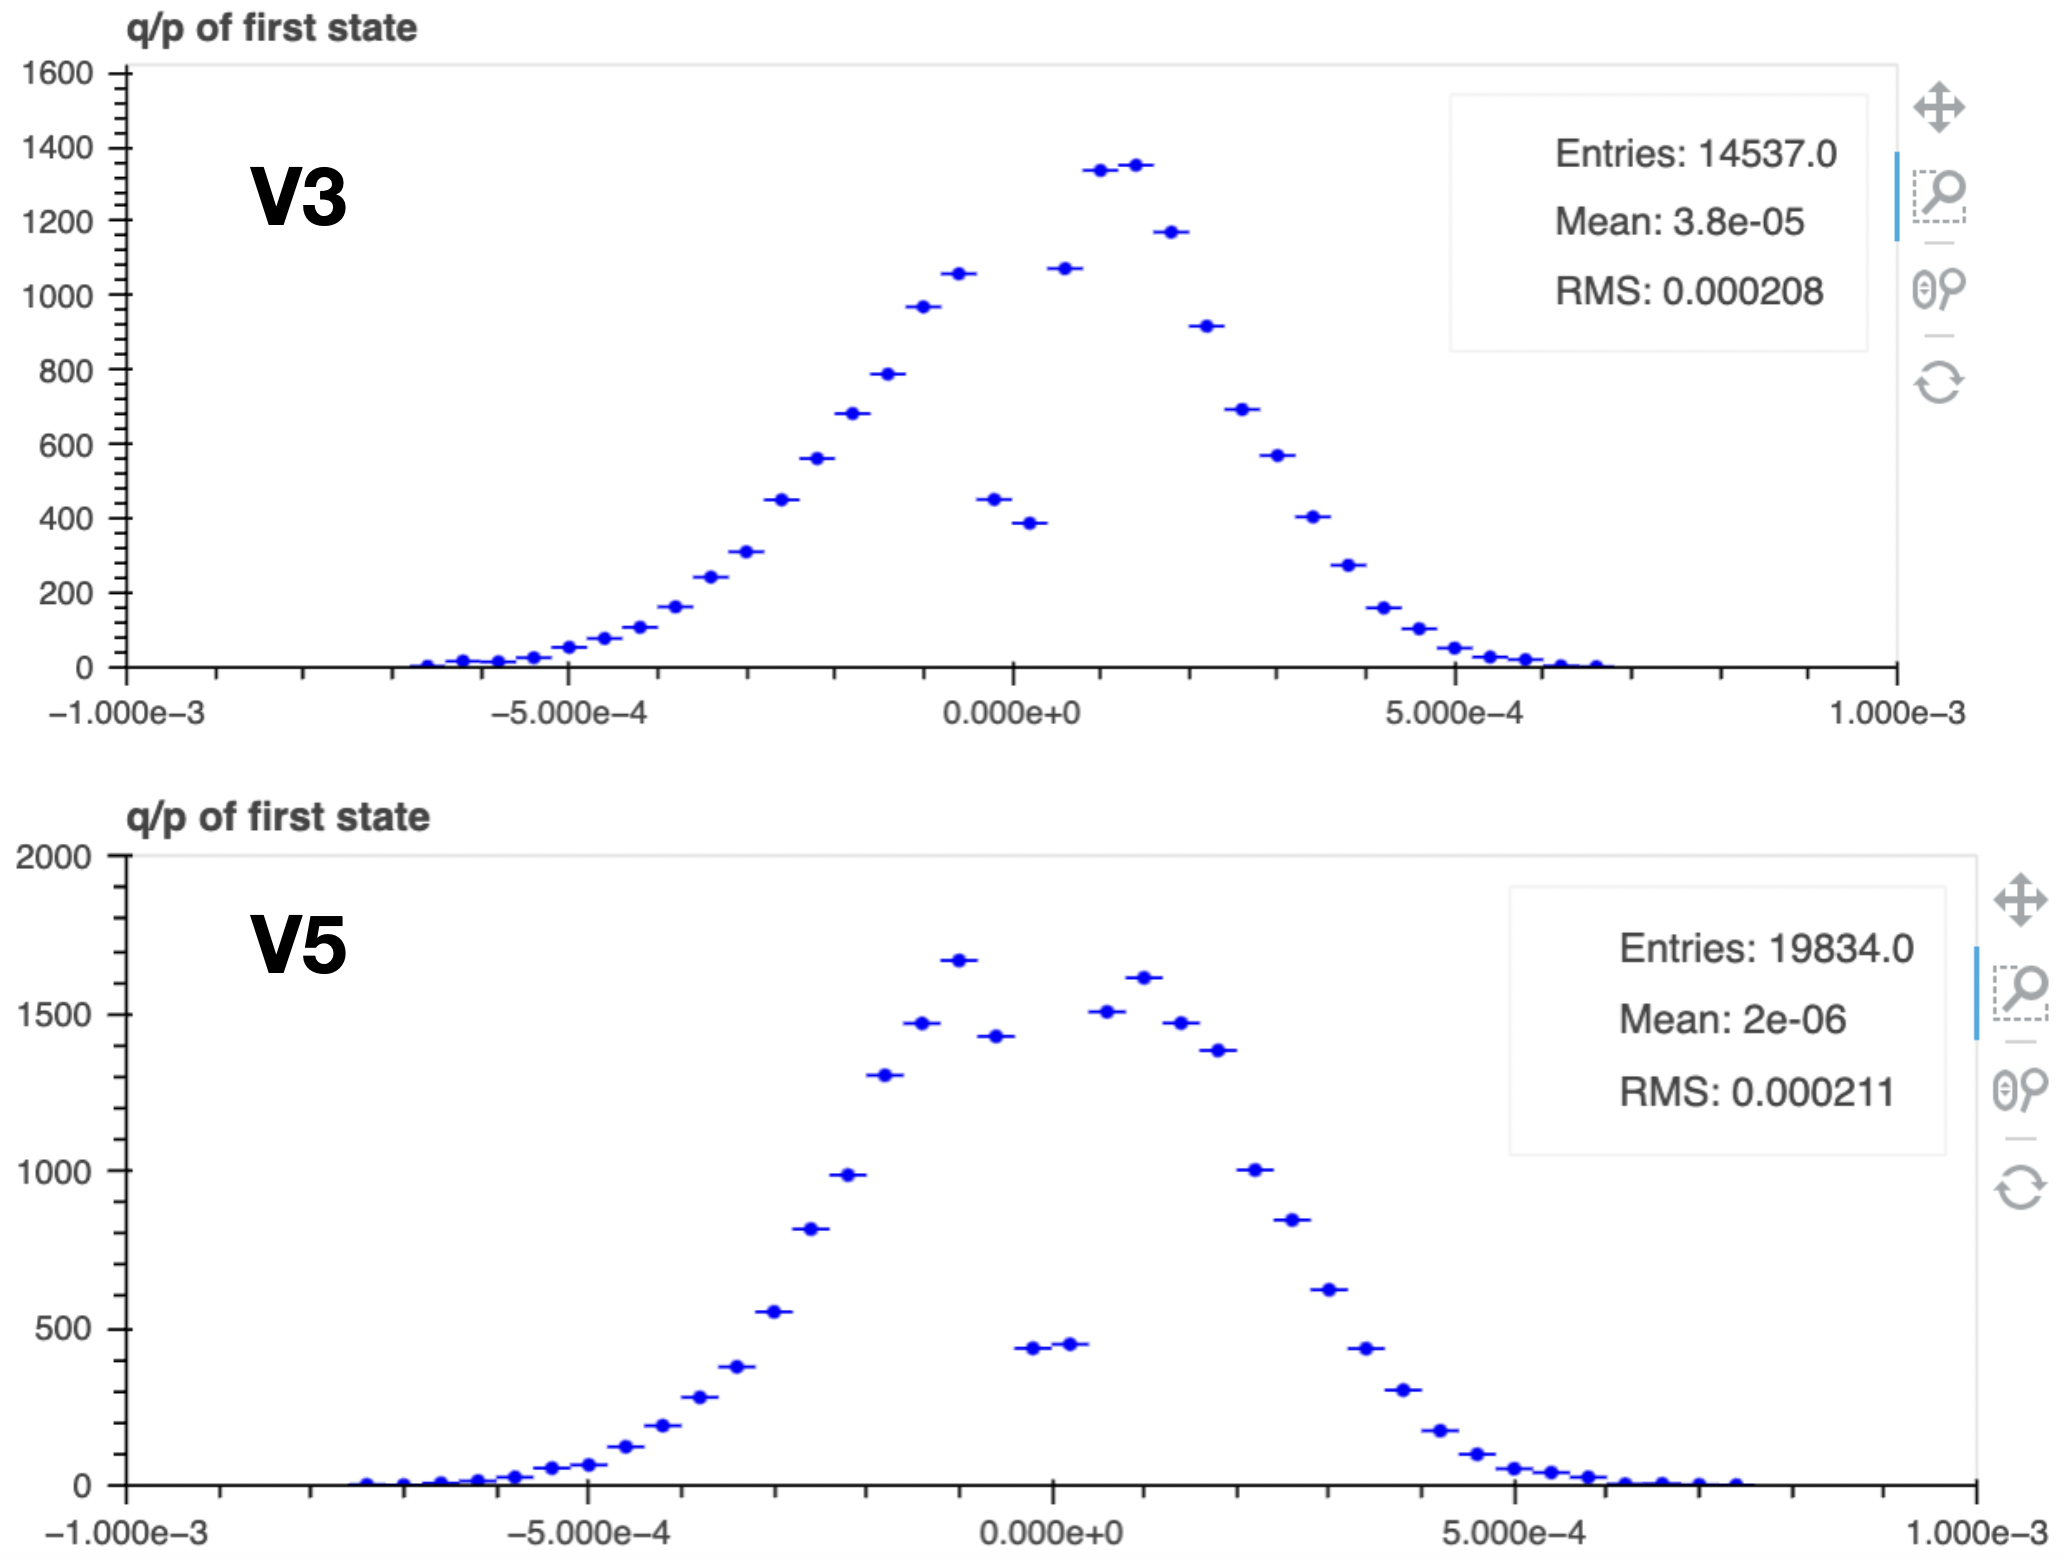
\includegraphics[width=0.5\textwidth]{plots/qop_v3v5.png}
      \end{figure}
    \end{column}
  \end{columns}  
\end{frame}

\begin{frame}\frametitle{Outlook}
  \begin{columns}
    \begin{column}[c]{0.55\textwidth}
      Alignment outlook in the coming months:
      \begin{itemize}
        \item $\bullet$\, Alignment stability and magnet up vs. magnet down tests in 2022 data (also later 2023 data)
        \item $\bullet$\, Dedicated MC studies for 2023 conditions and using what we have learned from 2022
        \item $\bullet$\, Continuing work with new data, commissioning SciFi alignment and the online alignment system
        \item $\bullet$\, Estimate SciFi alignment accuracy needed to trigger automatic update of constant and automatic alignment monitoring
      \end{itemize}
    \end{column}
    \begin{column}[c]{0.43\textwidth}
      sim+reco outlook:
      \begin{itemize}
      	\item $\bullet$\, Effort on Boole code modernization
	      \item $\bullet$\, Louis writing a note on cluster resolution
	      \item $\bullet$\, Louis also writing a definitive document about clusterization, encoding and decoding
      \end{itemize}
    \end{column}
  \end{columns}
\end{frame}

\end{document}
